\documentclass[glossaries, index]{kidiplom}

\title{Kryptoanalýza klasických šifer}
\title[english]{Cryptanalysis of classical ciphers}
\author{Josef Podstata}
\supervisor{\hfill \newline RNDr. Eduard Bartl, Ph.D.}
%\yearofsubmit{\the\year}

\keywords{šifra, kryptologie, kryptografie, kryptoanalýza, iOS}
\keywords[english]{cipher, cryptology, cryptography, cryptanalysis, iOS}

\annotation{Metody šifrování a luštění šifer několikrát změnily lidskou historii. Práce \mbox{rozebírá} algoritmy prolamování vybraných historických šifer bez znalosti šifrovacího klíče a zkoumá jejich efektivitu vzhledem k počtu znaků zašifrované zprávy.}
\annotation[english]{Methods of encryption and breaking ciphers have changed human history many times. This thesis analyzes code breaking algorithms of specific historical ciphers without knowing the key and their effectivity considering the text length.}

\thanks{Děkuji RNDr. Eduardu Bartlovi, Ph.D. za vedení práce a za cenné rady při konzultacích.}

%% Packages %%
\usepackage{amsmath}
\usepackage{gensymb}
\usepackage{graphicx}
\usepackage{tikz}
\usepackage{indentfirst}
\usepackage{fancyvrb}
\usepackage{natbib}


\hyphenation{stati-sti-ku}
\hyphenation{algo-ri-tmus}
\hyphenation{mono-alfa-be-ti-cké}



\begin{document}

%% Úvod %%
\maketitle


%%%% Introduction %%%%
\section{Úvod}
\label{introduction-section}
Šifrování jako nástroj pro utajení informací je velmi starou vědní disciplínou.
Nejstarší dochovalé záznamy o~použití šifer se datují až do starověkého Egyptu, kde se okolo roku 1900 př.~n.~l. používaly tajné hieroglify, které měly skrytý význam i~pro jinak gramotné obyvatele. Archeologické nálezy dále naznačují použití substitučních šifer v~Mezopotámii okolo 1500 př.~n.~l. a~nebo Číně okolo roku 1000 př.~n.~l.

 Kryptologie od té doby prošla velkým vývojem. Dnes jsou definované a~veřejně známé desítky šifrovacích postupů, které vznikly napříč lidkou historií. Největším vývojem prošla kryptologie během válečných konfliktů, kdy armáda jedné strany potřebovala zaručit bezpečnou komunikaci mezi vlastními jednotkami, ale znepřístupnit tajné informace druhé straně konfliktu, která mohla komunikaci odchytit.

Ke většině historických šifer se po letech objevily postupy, jak zašifrovaný text prolomit i~bez znalosti tajného klíče. Používání prolomené šifry se tedy stalo nebezpečným a~jako reakce na to se zvýšil zájem o~novější, bezpečnější způsoby šifrování.

Klasické šifrování, ke kterému stačí pouze tužka a papír, postupem času vymizelo a~dnes se téměř každý den setkáváme s~moderní kryptografií, ve které lze díky moderní elektronice dosáhnout daleko větší bezpečnosti.

Cílem práce je prozkoumat vybrané historické šifrovací algoritmy, vyzkoušet útoky kryptoanalytickými algoritmy na zašifrované zprávy a~změřit přibližnou úspěšnost těchto útoků.

\subsection{Definice základních pojmů}
\subsubsection{Kryptografie}
Kryptografie je věda zabývající se šifrovacími algoritmy.

\subsubsection{Kryptogranalýza}
Kryptoanalýza je věda zabývající se prolamováním šifrovacích algoritmů.

\subsubsection{Kryptologie}
Kryptologie je obecně věda zabývající se šifrováním. Zahrnuje kryptografii i~kryptoanalýzu.

\subsubsection{Otevřený text}
Text zprávy určené k~zašifrování. V~ukázkových příkladech této práce se píše malými písmeny.

\subsubsection{Zašifrovaný text}
Text zprávy zašifrovaný některým z~šifrovacích algoritmů. Člověku může připadat jako nesmyslná posloupnost náhodných znaků. Zašifrovaný text má v sobě stále ukryt původní otevřený text. Zpravidla se píše velkými písmeny.

\subsubsection{Šifrovací klíč}
Klíč může být libovolný znak, posloupnost znaků, číslo, nebo i~celá abeceda znaků. Záleží na zvolené šifře, každá definuje svou množinu možných klíčů. K~šifrování i~rozšifrování je klíč nezbytný a~spolu se zvolenou šifrou určuje přesný postup zašifrování otevřeného textu a~opačně i~pro rozšifrování.

\subsubsection{Šifra}
Šifrou se většinou rozumí šifrovací algoritmus, který z~otevřeného textu a~šifrovacího klíče vytvoří zašifrovanou zprávu, která je na první pohled nepochopitelná. Taková zpráva se může dostat ke komukoli, komu není určena, ale nebude ji schopen přečíst. Pouze pověřená osoba, pro kterou je zpráva určena, zná klíč i~použitou šifru a~pomocí inverzního algoritmu může zprávu rozšifrovat na původní čitelný text. Celý šifrovací proces ukazuje následující obrázek:

\begin{figure}[htbp]
\centering
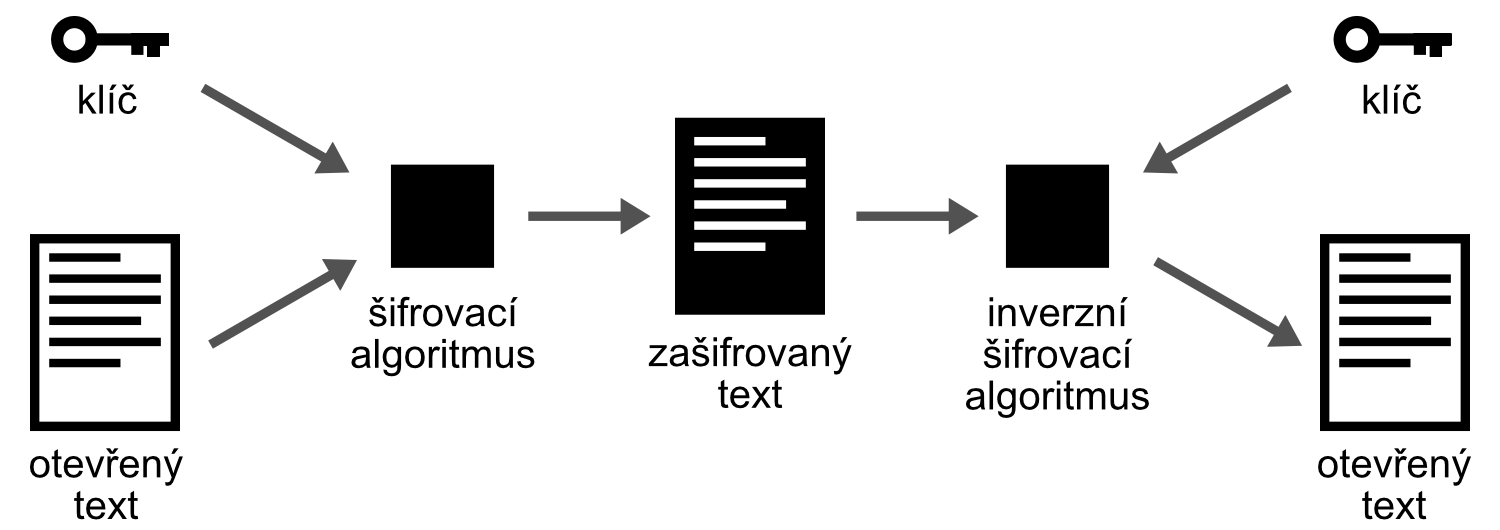
\includegraphics[scale=0.25]{graphics/encrypt_decrypt.png}
\caption{Proces šifrování a dešifrování}
\label{encrypting}
\end{figure}

Šifrovací algoritmus je tedy přesný popis jak text přepsat na nečitelný šifrovaný za použití určitého klíče. K~němu inverzní algoritmus popisuje přesně opačný proces. Oba algoritmy jsou většinou veřejně známé a~pouze klíč je tajná informace.

\subsubsection{Prolomení šifry}
Prolomení neboli rozluštění šifry znamená uhodnutí klíče ze samotného zašifrovaného textu. Slouží k~tomu vybraný prolamovací algoritmus, který text analyzuje a~vypočítá nejpravděpodobnější klíč. Proces ukazuje obrázek \ref{crackcode}.

\begin{figure}[htbp]
\centering
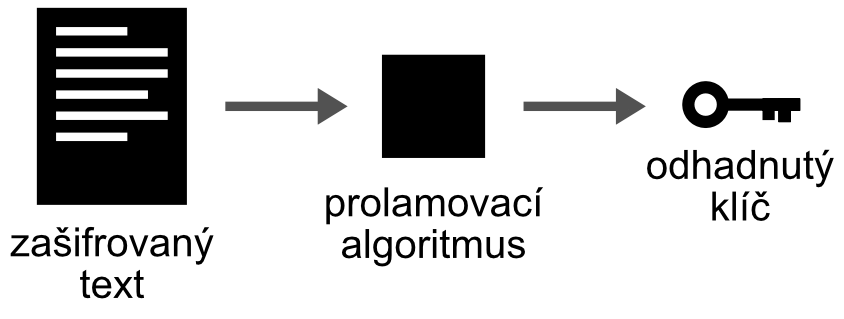
\includegraphics[scale=0.25]{graphics/cracking.png}
\caption{Proces prolomení šifry - získání klíče}
\label{crackcode}
\end{figure}

\subsubsection{Frekvenční analýza}
Frekvenční analýza je jedna ze základních kryptoanalytických metod. Jedná se o~výpočet jednotlivých znaků v~textu a~vytvoření procentuální statistiky, která určuje, jak často se které písmena v textu vyskytují.

\subsubsection{Bigramy, trigramy}
Bigramy jsou dvojice písmen jdoucí po sobě. Nápodobně trigramy trojice písmen. Pokud známe procentuálně nejpoužívanější bigramy a trigramy jazyka, můžeme je využít k posílení přesnoti algoritmů pracujících s frekvenční analýzou.

\subsubsection{Steganografie}
Stenografie je věda zabývající se ukrytím zpráv, aby k~nim neměl přístup nikdo nepověřený. Slovo pochází z řeckých \textit{steganos} (schovaný) a \textit{graphein} (psát)~\cite{singh2009}. Patří sem například psaní zpráv neviditelným inkoustem nebo zazdění kamené tabulky se zprávou. Ukryté texty většinou bývají navíc zašifrované.

\subsection{Typy šifer}
\subsubsection{Substituční šifry}
U substituční šifry je každý znak otevřeného textu nahrazen (substituován) na jiný znak nebo skupinu znaků. Většinou se definuje přepisovací (šifrovací) abeceda pro monoalfabetickou nebo více takových abeced pro polyalfabetickou šifru. Množina šifrovacích abeced společně s~původní abecedou zvoleného jazyka tvoří vše potřebné k~šifrování. 

Speciální případ je Vernamova šifra, jejíž klíč je stejně dlouhý jako otevřený text a~každý znak otevřeného textu se šifruje jiným znakem z~klíče.

\subsubsection{Transpoziční šifry}
Na rozdíl od substitučních šifer transpoziční nepřepisují znaky, ale pouze přehazují jejich pořadí. Šifrováním se nemění četnost znaků a~k~prolamování nelze použít klasické frekvenční analýzy. 

\subsubsection{Kombinované šifry}
Existují a~dodnes se používají také šifry, které kombinují postupy substitučních i transpozičních šifer dohromady. Zvýšenou složitostí algoritmů se zvyšuje i~bezpečnost. 

\subsubsection{Asymetrické šifry}
Všechny dosud probrané šifry jsou symetrické. Symetrické šifry používají k~šifrování i~rozšifrování stejný klíč. Asymetrické šifry používají dvojici klíčů, což markantně zvyšuje bezpečnost a~výpočetní náročnost. První klíč, tzv. veřejný, zašifruje zprávu a~druhý klíč, tzv. tajný, ji může zpátky rozšifrovat. Tajný klíč by měla mít k~dispozici pouze pověřená osoba.

S asymetrickými šiframi se dnes setkáváme v řadě případů, např. u elektronického podpisu, ukládání citlivých dat do databáze nebo pro ověření integrity. Dále se práce zabývá pouze šiframi symetrickými.

\vspace*{\fill}

\noindent
Zdroje k \ref{introduction-section}. kapitole: \cite{singh2009}, \cite{adams2003}, \cite{cryptographywiki}, \cite{cryptographywiki-en}, \cite{frequencyanalysiswiki}

\newpage


%%%% Caesar %%%%
\section{Caesarova šifra}
\label{caesar-section}
Caesarova šifra je jedna z~nejjednodušších variant monoalfabetické substituční šifry. Využívá posunutí původní abecedy o~předem určený počet míst, proto některé zdroje uvádí název \uv{posuvná šifra}. Také se může vyskytnout označení \uv{Caesarův kód}.

\subsection{Historie}
\label{caesar-history}
Šifra je pojmenovaná podle Římského politika a~vojevůdce Julia Caesara (100~př.~n.~l.~--~44~př.~n.~l.), který využíval šifru při psaní korespondence s~důvěrnými informacemi (např. týkající se vojenských tažení). Bezpečnost používání šifry byla v~té době vysoká, protože algoritmus nebyl veřejně známý a~hodně obyvatel ani nebylo gramotných. Caesar ale údajně používal i~jiné šifry.

Šifru můžeme také nalézt na některých Židovských mezuzách k zašifrování božských jmen. 
V roce 2006 byl usvědčen člen Sicilské mafie Cosa Nostra, protože vládní složky odchytili a~lehce prolomili členskou komunikaci. Používali modifikovanou Caesarovu šifru (písmena přepisovali na po sobě jdoucí čísla). Podobně v~roce 2011 byl Rajib Karim, bývalý zaměstnanec British Airways, usvědčen kvůli projednávání výbuchu letadel s~islámskými aktivisty, přičemž údajně použili Caesarovu šifru.

\subsection{Popis algoritmu}
\label{caesar-popis-algoritmu}
Algoritmus bere na vstupu text určený k~zašifrování (otevřený text) a~klíč ve tvaru jednoho písmene standartní abecedy. Z klíče se vypočítá délka posunu. Klíč 'A' značí posun o~nula pozic, 'B' o~jednu pozici atd.

Další postup se nejlépe ukáže na vypsání dvou abeced pod sebe, které společně ukazují všechny potřebné substituce. První z nich je původní abeceda používaného jazyka, druhá se nazývá šifrovací abeceda. Šifrovací abeceda se vytvoří posunutím původní o~počet pozic, který udává klíč. Písmena vysunutá za levý okraj abecedy rotují na konec. Příklad abeced pro klíč 'G':\\

\begin{center}
\begin{BVerbatim}
abcdefghijklmnopqrstuvwxyz
GHIJKLMNOPQRSTUVWXYZABCDEF
\end{BVerbatim}
\end{center}

V posledním kroku se každé písmeno otevřeného textu přepíše na příslušnou substituci podle posunuté abecedy a~takový text se vrátí. Příklad použití s klíčem 'G', kde první řádek značí otevřený text a~druhý řádek zašifrovaný text:\\

\begin{center}
\begin{BVerbatim}
"caesar je vazne nemocen"
"IGKYGX PK BGFTK TKSUIKT"
\end{BVerbatim}
\end{center}


Při ručním šifrování nám může pomoci jednoduchý šifrovací disk (též \uv{kruhový dekodér} z~anglického \uv{ring decoder}), což je nástroj složený ze dvou kruhů, kde na každém kruhu je vypsaná abeceda. Vnější abeceda je šifrovací, s~kruhem lze otáčet a~tím měnit klíč.

\begin{figure}[htbp]
\centering
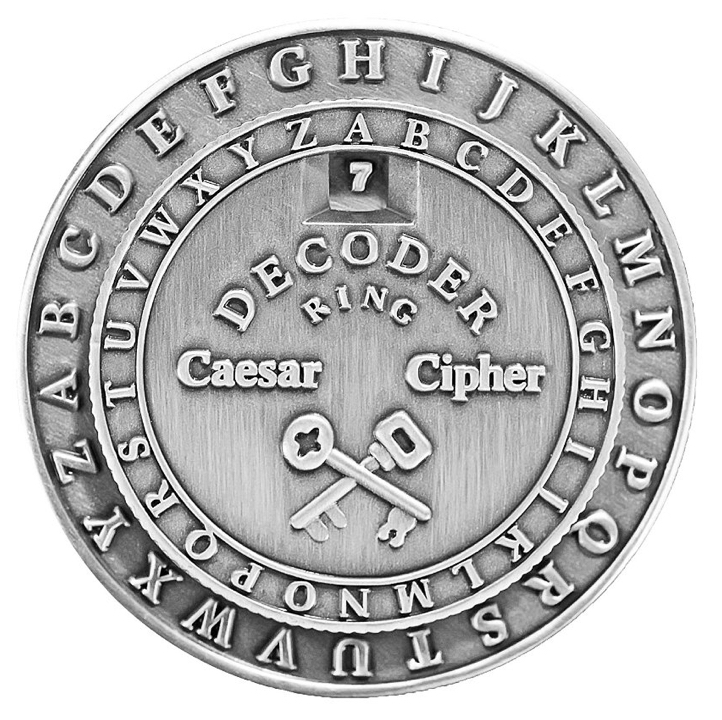
\includegraphics[scale=0.2]{graphics/ring_decoder.jpg}
\caption{Šifrovací disk k Caesarově šifře \cite{cipherdisk}}
\end{figure}

\subsection{Výhody}
Casarova šifra je jednoduchá na pochopení i~použití. Jako pomůcku pro zrychlení můžeme využít šifrovací disk nebo prsten.

\subsection{Nevýhody}
Existuje pouze tolik možných klíčů, kolik je znaků v abecedě. Typicky pro anglickou abecedu pouze 26 znaků. Z toho znak 'A' je tzv. slabý klíč, který po zašifrování otevřený text ani nepozmění. Šifrovaný text lze prolomit bez dodatečných pomůcek v~řádu minut tím, že jednoduše vyzkoušíme všechny možné klíče.

\subsection{Prolamování}
\subsubsection{Útok hrubou silou pomocí frekvenční analýzy}
\label{caesar-frekvencni-analyza}
Tento algoritmus využívá slabiny obecně všech monoalfabetických šifer, že ze zašifrovaného textu se dá vypočítat procentuální výskyt použitých znaků. Z~každého jazyka se dá vytvořit statistika udávající procentuální výskyt znaků, bigramů, trigramů atd.

První musíme znát předpokládaný výskyt všech písmen abecedy v~daném jazyce, s~kterým pracujeme. Pro češtinu ji znázorňuje graf na obrázku \ref{czech-frequency-analysis}. Poté sestavíme obdobnou statistiku ze zašifrovaného textu. Inicialuzjeme pole s~tolika prvky, kolik je znaků v abecedě. Všechny prvky jsou na počátku nuly. Projdeme celý zašifrovaný text a~s~každým výskytem písmene inkrementujeme o~jedna příslušný prvek v~poli. Nakonec každý prvek vydělíme počtem znaků v~zašifrovaném textu a~máme procentuální četnost znaků. 
 
\begin{figure}[htbp]
\centering
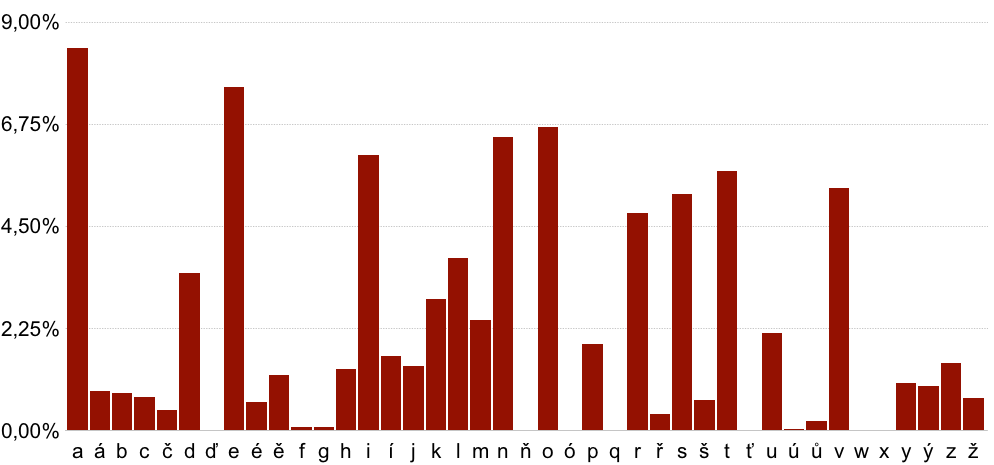
\includegraphics[scale=0.42]{graphics/czech_frequency.png}
\caption{Přibližná četnost znaků v českém textu \cite{letterfrequencywiki}}
\label{czech-frequency-analysis}
\end{figure}

Při luštění na papíře stačí porovnat vypočítanou statistiku se statistikou jazyka. Pro obě statistiky nakreslíme přibližný graf a~položíme je pod sebe. Poté posouváme grafem nalevo nebo napravo a hledáme pozici, kde se budou grafy vertikálně nejvíc podobat. 

Pro program je postup jiný. Zašifrovaný text postupně rozšifruje každým možným klíčem a~výsledný rozšifrovaný text podrobí frekvenční analýze. Tuto statistiku porovná s~předpokládanou statistikou daného jazyka a~vypočítá odchylku. Odchylka nyní určuje podobnost zvoleného klíče s~hledaným klíčem. Postup se opakuje pro všechny klíče a~algoritmus vybere ten z~nich, pro který vypočítal nejmenší odchylku. Takový klíč vrátí na výstupu. Úspěšnost algoritmu vzhledem k~počtu znaků zašifrované zprávy ukazuje graf na obrázku \ref{caesar-frequency-analysis}.

\begin{figure}[htbp]
\centering
\begin{tikzpicture}[x=0.06cm,y=0.18cm]
  \def\xmin{25}
  \def\xmax{150}
  \def\ymin{80}
  \def\ymax{100}
  \draw[style=help lines, ystep=10, xstep=25] (\xmin,\ymin) grid
  (\xmax,\ymax);
  \draw[->] (\xmin,\ymin) -- (\xmax+6,\ymin) node[right] {$characters$};
  \draw[->] (\xmin,\ymin) -- (\xmin,\ymax+2) node[above] {$success$};
  \foreach \x in {25,50,...,150}
    \node at (\x, \ymin-0.5) [below] {\x};
  \foreach \y in {80,90,...,100}
    \node at (\xmin-1.5,\y) [left] {\y \%};
  \draw[color={rgb:red,221;green,45;blue,54}] plot[smooth,tension=0.3,mark=*,mark size=1pt] file {data/Caesar-frequency_analysis.dat}
   node [right] {frequency analysis};
\end{tikzpicture}
\caption{Úspěšnost frekvenční analýzy na Caesarovu šifru}
\label{caesar-frequency-analysis}
\end{figure}

Algoritmus používá pouze základní verzi frekvenční analýzy, kde se pracuje jen s~jednotlivými znaky. Vylepšení algoritmu je možné například přidáním počítání bigramů a~trigramů.

\subsubsection{Útok hrubou silou hledáním reálných slov}
Tento algoritmus také postupně zkouší všechny přijatelné klíče. Pro vypočítání úspěšnosti jednotlivých klíčů využívá seznam nejpoužívanějších slov daného jazyka. 

Každým klíčem rozšifrujeme text a~poté u~něho spočítáme počet výskytů jednotlivých slov ze seznamu nejpoužívanějších slov. Výskyty slov sečteme. Součet udává úspěšnost aktuálně zkoušeného klíče. Postup zopakujeme pro každý klíč a~nakonec vybereme ten nejúspěšnější. Úspěšnost s~použitím seznamu o~100 nejpoužívanějších slovech ukazuje graf na obrázku \ref{caesar-real-words}. 

\begin{figure}[htbp]
\centering
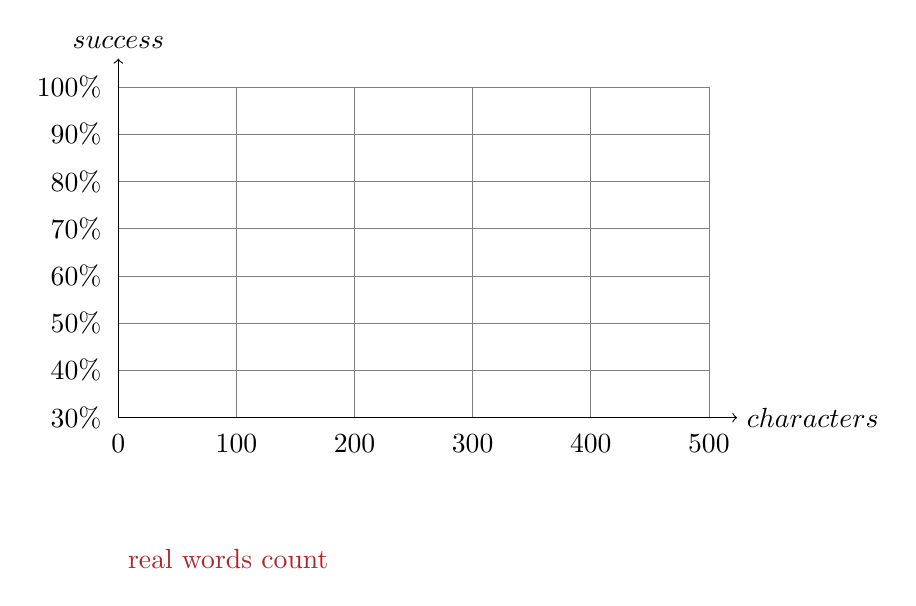
\begin{tikzpicture}[x=0.015cm,y=0.06cm]
  \def\xmin{0}
  \def\xmax{500}
  \def\ymin{30}
  \def\ymax{100}
  \draw[style=help lines, ystep=10, xstep=100] (\xmin,\ymin) grid
  (\xmax,\ymax);
  \draw[->] (\xmin,\ymin) -- (\xmax+24,\ymin) node[right] {$characters$};
  \draw[->] (\xmin,\ymin) -- (\xmin,\ymax+6) node[above] {$success$};
  \foreach \x in {0,100,...,500}
    \node at (\x, \ymin-1.5) [below] {\x};
  \foreach \y in {30,40,...,100}
    \node at (\xmin-6,\y) [left] {\y \%};
  \draw[color={rgb:red,221;green,45;blue,54}] plot[smooth,tension=0.3,mark=*,mark size=1pt] file {data/Caesar-real_words.dat}
   node [right] {real words count};
\end{tikzpicture}
\caption{Úspěšnost útoku hledáním reálných slov na Caesarovu šifru}
\label{caesar-real-words}
\end{figure}

\subsubsection{Trojúhelníkový útok}
--- dopsat ---

Lorem ipsum dolor sit amet. Lorem ipsum dolor sit amet. Lorem ipsum dolor sit amet. Lorem ipsum dolor sit amet. Lorem ipsum dolor sit amet. Lorem ipsum dolor sit amet. Lorem ipsum dolor sit amet. Lorem ipsum dolor sit amet. Lorem ipsum dolor sit amet. Lorem ipsum dolor sit amet. Lorem ipsum dolor sit amet. Lorem ipsum dolor sit amet. Lorem ipsum dolor sit amet. Lorem ipsum dolor sit amet. Lorem ipsum dolor sit amet. Lorem ipsum dolor sit amet. Lorem ipsum dolor sit amet. Lorem ipsum dolor sit amet. Lorem ipsum dolor sit amet. Lorem ipsum dolor sit amet. Lorem ipsum dolor sit amet. Lorem ipsum dolor sit amet. Lorem ipsum dolor sit amet. Lorem ipsum dolor sit amet. Lorem ipsum dolor sit amet. Lorem ipsum dolor sit amet. Lorem ipsum dolor sit amet. Lorem ipsum dolor sit amet. Lorem ipsum dolor sit amet. Lorem ipsum dolor sit amet. 

Lorem ipsum dolor sit amet. Lorem ipsum dolor sit amet. Lorem ipsum dolor sit amet. Lorem ipsum dolor sit amet. Lorem ipsum dolor sit amet. Lorem ipsum dolor sit amet. Lorem ipsum dolor sit amet. Lorem ipsum dolor sit amet. Lorem ipsum dolor sit amet. Lorem ipsum dolor sit amet. Lorem ipsum dolor sit amet. Lorem ipsum dolor sit amet. Lorem ipsum dolor sit amet. Lorem ipsum dolor sit amet. Lorem ipsum dolor sit amet. Lorem ipsum dolor sit amet. Lorem ipsum dolor sit amet. Lorem ipsum dolor sit amet. 

\begin{figure}[htbp]
\centering
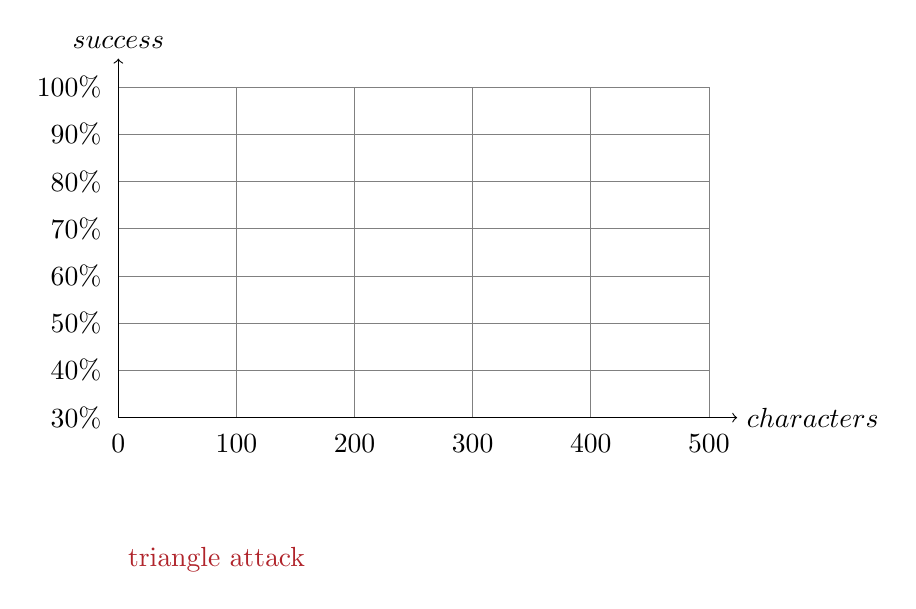
\begin{tikzpicture}[x=0.015cm,y=0.06cm]
  \def\xmin{0}
  \def\xmax{500}
  \def\ymin{30}
  \def\ymax{100}
  \draw[style=help lines, ystep=10, xstep=100] (\xmin,\ymin) grid
  (\xmax,\ymax);
  \draw[->] (\xmin,\ymin) -- (\xmax+24,\ymin) node[right] {$characters$};
  \draw[->] (\xmin,\ymin) -- (\xmin,\ymax+6) node[above] {$success$};
  \foreach \x in {0,100,...,500}
    \node at (\x,\ymin-1.5) [below] {\x};
  \foreach \y in {30,40,...,100}
    \node at (\xmin-6,\y) [left] {\y \%};
  \draw[color={rgb:red,221;green,45;blue,54}] plot[smooth,tension=0.3,mark=*,mark size=1pt] file {data/Caesar-triangle_attack.dat}
   node [right] {triangle attack};
\end{tikzpicture}
\caption{Úspěšnost trojúhelníkového utoku na Caesarovu šifru}
\end{figure}

\vspace*{\fill}

\noindent
Zdroje ke \ref{caesar-section}. kapitole: \cite{singh2009}, \cite{stinson2006}, \cite{caesarwiki}, \cite{caesarwiki-en}, \cite{letterfrequencywiki}

\newpage


%%%% Vigenere %%%%
\section{Vigenèrova šifra}
\label{vigenere-section}
Vigenèrova šifra je polyalfabetická (využívající více šifrovacích abeced) substituční šifra. Písmena se sice šifrují stejným způsobem jako u~Caesarovy šifry, ale po každém substituovaném písmenu se změní šifrovací abeceda. Celý postup se tedy skládá z~postupné aplikace několika různých Caesarových šifer.

\subsection{Historie}
Šifra je nesprávně pojmenovaná po francouzském diplomatovi a kryptografovi jménem Blaise de Vigenère, který roku 1586 publikoval popis podobné, ale silnější šifry. Název Vigenèrova šifra se začal mylně používat až v~19. století.

Nejstarší dochovalý popis šifry je z~roku 1467, kdy italský matematik Leon Battista Alberti popsal velmi podobnou polyalfabetickou šifru. Šifrovací abecedu ale nemění po každém znaku, nýbrž až po celých slovech nebo i~větách. 

V roce 1508 Němec Johannes Trithemius vynalezl Vigenèrův čtverec (známý také jako Vigenèrova tabulka), tedy pomůcku k šifrování znázorňující všech 26 použitelných šifrovacích abeced. Původní latinský název je \uv{tabula recta}.

\begin{figure}[htbp]
\centering
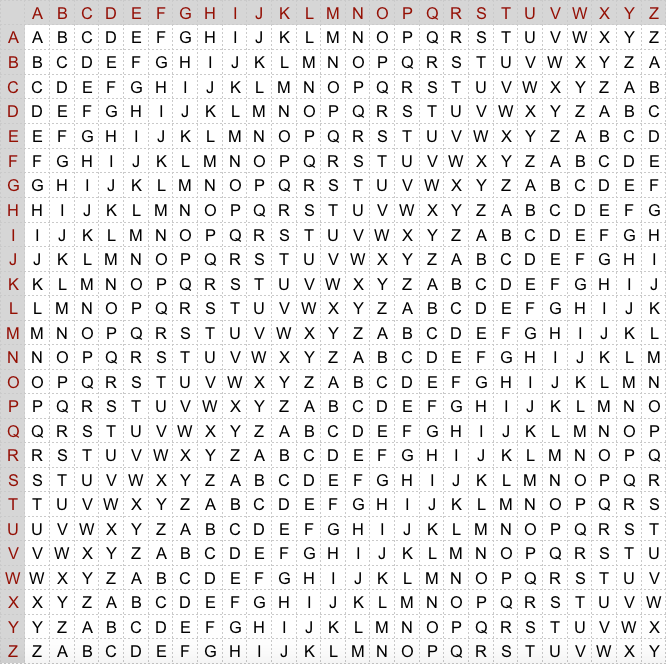
\includegraphics[scale=0.4]{graphics/vigenere_square.png}
\caption{Vigenèrův čtverec}
\label{vigenere-square}
\end{figure}

Šifru, kterou dnes chápeme pod pojmenováním Vigenèrova šifra, přesně popsal Giovan Battista Bellaso ve svém díle \textit{La cifra del. Sig. Giovan Battista Bellaso} z~roku 1553. Využil už existující Vigenèrův čtverec a~definoval klíč o~více znacích (například slovo nebo krátká fráze), díky kterému se jasně střídají šifrovací abecedy po každém přepsaném znaku.

Šifra se prakticky začala používat až daleko později, protože na svou dobu byla moc složitá. Velmi dlouho byla považována za nerozluštitelnou. V roce 1863 publikoval německý kryptoanalytik Friedrich Wilhelm Kasiski práci, ve které popisuje prolomení \uv{neprolomitelné} Vigenèrovy šifry. Byl to sice první publikovaný popis prolomení, ale britský matematik Charles Babbage prolomil tuto šifru už daleko dřív v~roce 1854, pouze svou práci nezveřejnil.

Vigenèrova šifra byla použita jako vojenská polní šifra v~Americké občanské válce (1861--1865) stranou států Konfederace. Státy Unie jako druhá strana konfliktu pravidelně prolamovali odchycené zašifrované zprávy.

\subsection{Popis algoritmu}
Algoritmus bere na vstupu otevřený text a klíč ve tvaru libovolně dlouhé posloupnosti znaků. Klíčem je většinou nějaké slovo používaného jazyka, aby si ho jednoduše zapamatovaly obě strany komunikace.

Podle prvního písmene z~klíče vytvoříme šifrovací abecedu stejně jako u~Caesarovy šifry. Takovou šifrovací abecedou zašifrujeme první písmeno otevřeného textu. Následuje stejný postup pro druhé písmeno klíče a~druhé písmeno otevřeného textu. To se opakuje pro všechny znaky klíče. Po posledním znaku klíče se zase začíná od prvního a~postup se opakuje dokud nezašifrujeme všechny znaky otevřeného textu.

\subsubsection{Příklad}
Zprávu \uv{lidska povaha je plna rozporu} zašifrujeme klíčem \uv{capek}. Aktuální šifrovací abecedu vždy vidíme ve Vigenerově čtverci. 

První zvolená šifrovací abeceda je podle znaku \uv{c}, tedy 3. řádek čtverce. V~ní se první písmeno otevřeného textu \uv{l} zašifruje na \uv{N}. Další šifrovací abeceda je \uv{a}, tedy stejná jako původní. Znak \uv{i} se v ní zobrazí na \uv{I}. Třetí abeceda je podle znaku \uv{p}, tedy 16. řádek čtverce. Znak \uv{d} se v ní zobrazí na \uv{S}. 

Po zašifrování celého textu stejným způsobem dostaneme výsledný zaširovaný text \uv{NISWUC PDZKJA YI ZNNP VYBPDVE}.

\subsection{Výhody}
Šifra je daleko bezpečnější bež většina monoalfabetických šifer nebo její polyalfabetičtí předchůdci. Přijímá tak velké množství možných klíčů, že útok hrubou silou je i~pro dnešní počítače neřešitelný v rozumném čase. I~pro poměrně krátký klíč o~$7$ znacích by to znamenalo $26^7$ možností, tedy $8$ miliard možných klíčů.

Další výhodou je odolnost proti frekvenční analýze. Samotná četnost znaků nebo bigramů zašifrovaného textu nenese žádnou důležitou informaci, které by se při prolamování dalo využít.

\subsection{Nevýhody}
Složitost šifry odrazuje od jejího použítí. Bez pomocného Vigenèrova čtverce nebo alespoň šifrovacího disku je proces šifrování na papíře velmi zdlouhavý.

Použití klíče o jednom znaku znamená použití obyčejné Caesarovy šifry. Také znak \uv{a} v~klíči šifru oslabuje.

Později se objevily slabiny využitelné při kryptoanalýze, například hledání skupin stejných po sobě jdoucích znaků k~určení délky klíče. Také můžeme využít předpokladu, že většina klíčů tvoří reálná slova a~ne pouze náhodné  znaky.

\subsection{Prolamování}
\subsubsection{Odhadnutí délky klíče}
\label{vigenere-delka_klice}
Délku klíče odhadneme pomocí výskytu stejných shluků znaků v zašifrovaném textu. V~otevřeném textu se může vyskytovat stejné slovo vícekrát. Předpokládáme, že se některá z takových slov zašifrovaly stejným způsobem. Například poměrně časté slovo \uv{nebo} se v~českém textu pravděpodobně objeví více jak jednou. Při zašifrování klíčem o~délce 6 je pouze 6 možností, jak se takové slovo zašifrovalo. Jeho 7. výskyt už určitě prozradí možnou délku klíče.

V prvním kroce si sestavíme seznam možných délek klíče. Při luštění na papíře bychom čísla vypsali pod sebe. Program si inicializuje pole \texttt{divisors} a všechny jeho prvky nastaví na číslo 0. Předpokládáme, že délka klíče se pohybuje mezi 4 až 10 znaky. Pole \texttt{divisors} tedy bude mít 7 prvků.

V~zašifrovaném textu postupně nalezneme všechny shluky znaků o~délce $n$, kde~$n \in \{4, 5, 6, 7\}$, které se v~textu vyskytují více jak jednou. Pro $n < 4$ můžeme nalézt rozdílné sekvence otevřeného textu zašifrované jinou částí klíče, které náhodou dávají stejný zašifrovaný výsledek (z knihy \cite{singh2009}). Z jejich vzdálenosti vypočítáme všechny dělitele. Každý takový dělitel je možná délka klíče. Množinu dělitelů omezíme minimální a~maximální předpokládanou délkou klíče. Poté pro každý dělitel inkrementujeme příslušný prvek v~poli \texttt{divisors} o~1. 

Po zpracování všech stejných shluků se z pole \texttt{divisors} vybere dělitel, který má nejvyšší hodnotu a~vyskytl se tedy nejvícekrát. Pokud je v~poli více prvků s~nejvyšší hodnotou, můžeme si vybrat, jestli předpokládáme výskyt krátkého, nebo dlouhého klíče. Úspěšnost uhodnutí délky klíče pro generované klíče v~rozmezí 4 až 10 znaků ukazuje graf na obrázku \ref{vigenere-key-length}.

\begin{figure}[htbp]
\centering
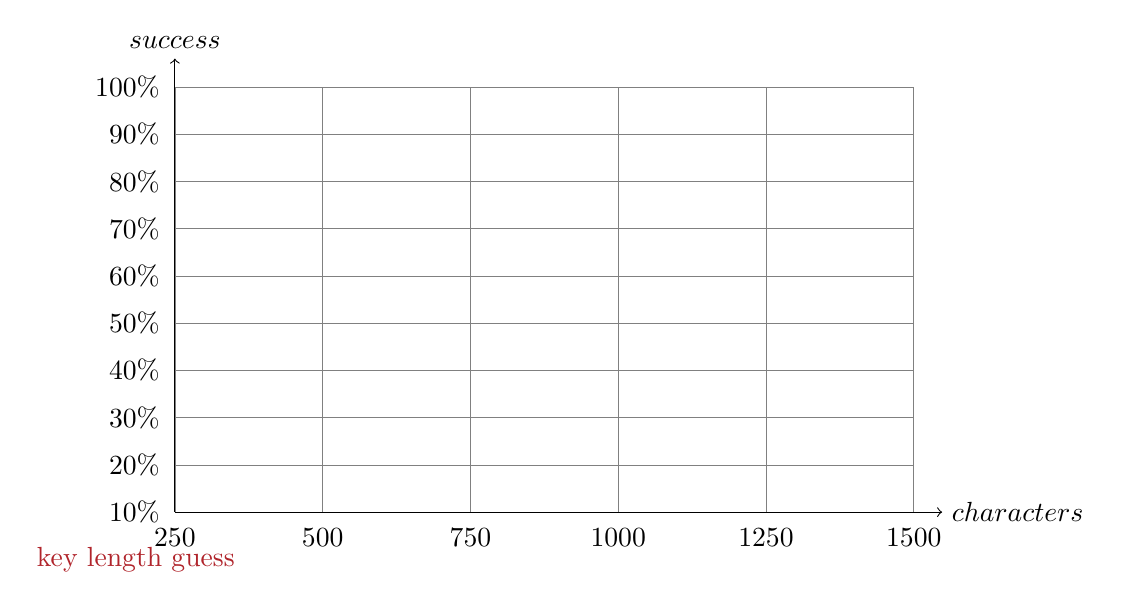
\begin{tikzpicture}[x=0.0075cm,y=0.06cm]
  \def\xmin{250}
  \def\xmax{1500}
  \def\ymin{10}
  \def\ymax{100}
  \draw[style=help lines, ystep=10, xstep=250] (\xmin,\ymin) grid
  (\xmax,\ymax);
  \draw[->] (\xmin,\ymin) -- (\xmax+48,\ymin) node[right] {$characters$};
  \draw[->] (\xmin,\ymin) -- (\xmin,\ymax+6) node[above] {$success$};
  \foreach \x in {250,500,...,1500}
    \node at (\x,\ymin-1.5) [below] {\x};
  \foreach \y in {10,20,...,100}
    \node at (\xmin-9,\y) [left] {\y \%};
  \draw[color={rgb:red,221;green,45;blue,54}] plot[smooth,tension=0.3,mark=*,mark size=1pt] file {data/Vigenere-key_length.dat}
   node [right] {key length guess};
\end{tikzpicture}
\caption{Úspěšnost odhadnutí délky klíče u Vigenèrovy šifry}
\label{vigenere-key-length}
\end{figure}

\subsubsection{Útok pomocí frekvenční analýzy}
Pomocí algoritmu \ref{vigenere-delka_klice} zjistíme nejpravděpodobnější délku klíče a~označíme ji $k$. Kdybychom délku klíče nemohli přesně určit, můžeme využít hrubé síly. Následující postup by se tak zopakoval pro každé $k$ z množiny definované minimálním a maximálním počtem znaků klíče.

Zašifrovaný text $T$ o délce $n$ rozdělíme na $k$ posloupností písmen. Pro každou posloupnost $P_{i}$ platí:
$$P_{i}[j] = S[i+j\times k]$$
\noindent
Pro $0 \leq i < k$ a zároveň $0 \leq (i+j\times k) < n$, kde $X[y]$ vrací $y$-tý znak řetězce $X$.

Nyní máme v~každé posloupnosti $P_{i}$ takové znaky zašifrovaného textu, které se zašifrovaly stejnou šifrovací abecedou. Pro každou posloupnost zavoláme algoritmus pracující s~frekvenční analýzou (viz. \ref{caesar-frekvencni-analyza} na straně \pageref{caesar-frekvencni-analyza}) a~zjistíme klíč, kterým byly znaky posloupnosti pravděpodobně zašifrovány. 

Výsledný klíč zašifrovaného textu se postupně složí z~výsledků frekvenční analýzy na každé posloupnosti $P_{i}$. Úspěšnost útoku ukazuje graf na obrázku~\ref{vigenere-frequency-analysis}. 

Při měření program generoval klíče o maximální délce 7 znaků. Pro menší maximální délku klíče jsou výsledky příznivější, pro větší naopak nepříznivější.

\begin{figure}[htbp]
\centering
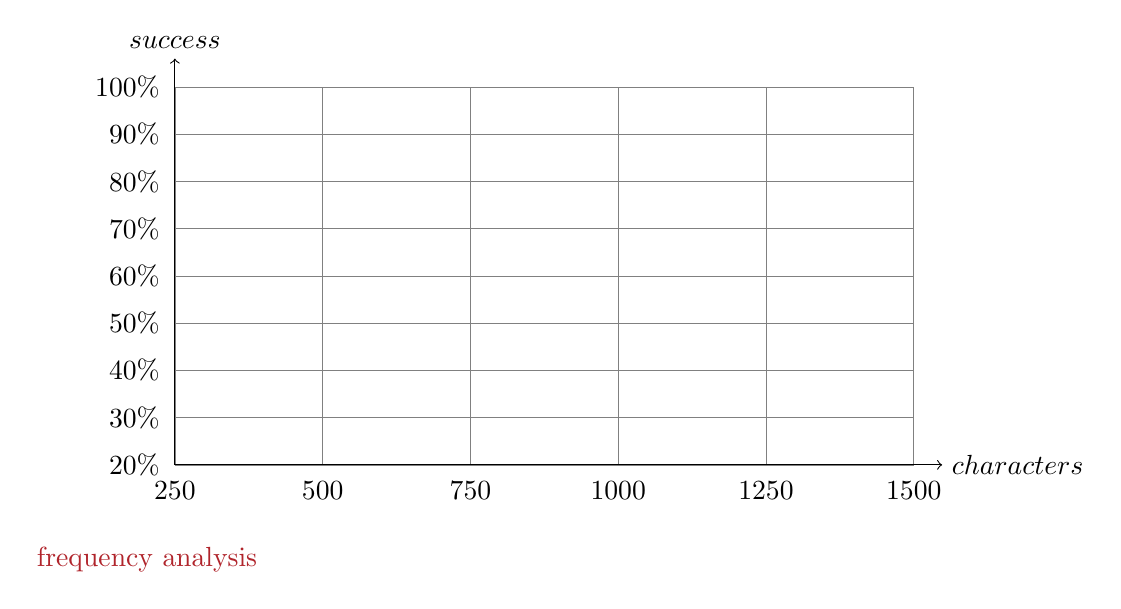
\begin{tikzpicture}[x=0.0075cm,y=0.06cm]
  \def\xmin{250}
  \def\xmax{1500}
  \def\ymin{20}
  \def\ymax{100}
  \draw[style=help lines, ystep=10, xstep=250] (\xmin,\ymin) grid
  (\xmax,\ymax);
  \draw[->] (\xmin,\ymin) -- (\xmax+48,\ymin) node[right] {$characters$};
  \draw[->] (\xmin,\ymin) -- (\xmin,\ymax+6) node[above] {$success$};
  \foreach \x in {250,500,...,1500}
    \node at (\x,\ymin-1.5) [below] {\x};
  \foreach \y in {20,30,...,100}
    \node at (\xmin-9,\y) [left] {\y \%};
  \draw[color={rgb:red,221;green,45;blue,54}] plot[smooth,tension=0.3,mark=*,mark size=1pt] file {data/Vigenere-frequency_analysis.dat}
   node [right] {frequency analysis};
\end{tikzpicture}
\caption{Úspěšnost frekvenční analýzy na Vigenèrovu šifru}
\label{vigenere-frequency-analysis}
\end{figure}

\subsubsection{Trojúhelníkový útok}
--- dopsat ---

Lorem ipsum dolor sit amet. Lorem ipsum dolor sit amet. Lorem ipsum dolor sit amet. Lorem ipsum dolor sit amet. Lorem ipsum dolor sit amet. Lorem ipsum dolor sit amet. Lorem ipsum dolor sit amet. Lorem ipsum dolor sit amet. Lorem ipsum dolor sit amet. 

\begin{figure}[htbp]
\centering
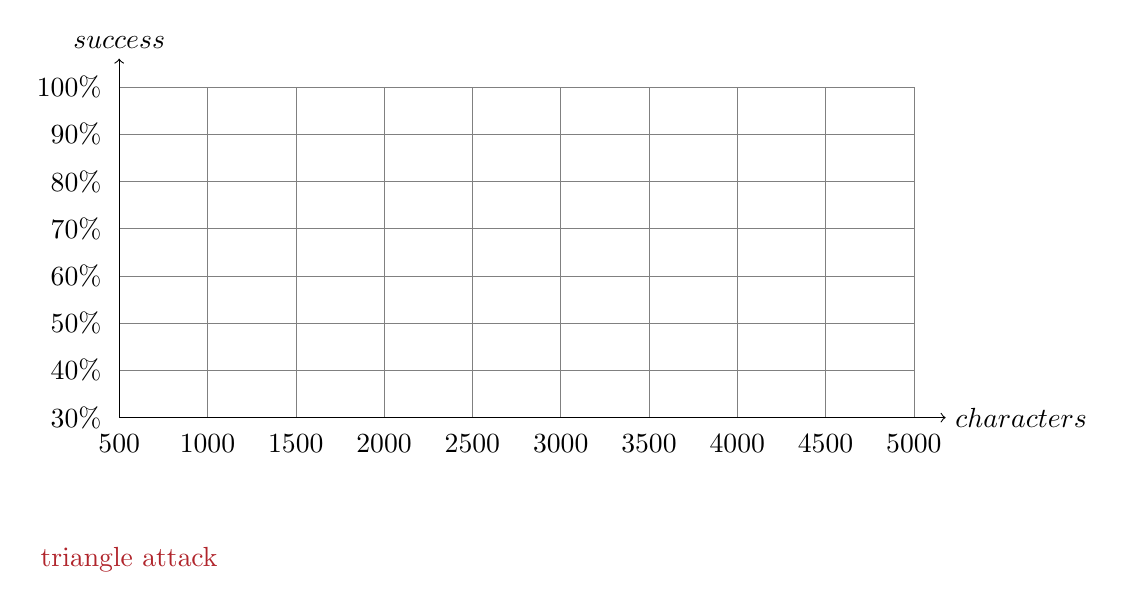
\begin{tikzpicture}[x=0.00225cm,y=0.06cm]
  \def\xmin{500}
  \def\xmax{5000}
  \def\ymin{30}
  \def\ymax{100}
  \draw[style=help lines, ystep=10, xstep=500] (\xmin,\ymin) grid
  (\xmax,\ymax);
  \draw[->] (\xmin,\ymin) -- (\xmax+180,\ymin) node[right] {$characters$};
  \draw[->] (\xmin,\ymin) -- (\xmin,\ymax+6) node[above] {$success$};
  \foreach \x in {500,1000,...,5000}
    \node at (\x,\ymin-1.5) [below] {\x};
  \foreach \y in {30,40,...,100}
    \node at (\xmin-45,\y) [left] {\y \%};
  \draw[color={rgb:red,221;green,45;blue,54}] plot[smooth,tension=0.3,mark=*,mark size=1pt] file {data/Vigenere-triangle_attack.dat}
   node [right] {triangle attack};
\end{tikzpicture}
\caption{Úspěšnost trojúhelníkového útoku na Vigenèrovu šifru}
\end{figure}

\vspace*{\fill}

\noindent
Zdroje ke \ref{vigenere-section}. kapitole: \cite{singh2009}, \cite{vigenerewiki}, \cite{vigenerewiki-en}, \cite{stinson2006}

\newpage


%%%% Monoalphabetic %%%%
\section{Obecná monoalfabetická šifra}
\label{monoalphabetic-section}
Základní monoalfabetická substituční šifra používá jako klíč libovolnou kompletní šifrovací abecedu. Proto je zobecněním pro několik dalších substitučních šifer, například pro Caesarovu nebo afinní šifru, které mají daleko jednodušší a~snadněji zapamatovatelné klíče, podle kterých se následně celá šifrovací abeceda dopočítá.

\subsection{Historie}
Do historie monoalfabetických šifer tedy patří i~historie Caearovy šifry (\ref{caesar-history}). Ještě starší záznamy ukazují použití hebrejské šifry Atbaš. Ta je speciální podobu monoalfabetické šifry, která jako šifrovací abecedu používá převrácenou původní. Znak 'a' se tedy zašifruje na 'Z', 'b'~na~'Y' atd. Šifra tedy neuvažuje žádný klíč, protože vždy používá jen jeden. Byla použita ve starých biblických textech z~\textit{Knihy Jeremjášovy} z~6. století př.~n.~l. \cite{atbashcipher}.

Šifrování bylo hojně používáno Araby v~době zlatého věku islámské civilizace. Kniha \textit{Adab al-Kuttáb} (Příručka úředníkova) z~10. století obsahuje pasáže o~šifrování monoalfabetickou šifrou, kde kromě náhodně uspořádaných písmen používali v~šifrovací abecedě i~jiné symboly než písmena \cite{singh2009}. Arabové také položili základy kryptografie.

Francie v~16. století odchytávala španělské zprávy šifrované monoalfabetickou šifrou. Španělská kryptoanalýza byla v~té době na velmi nízké úrovni. Francouzi už dávno věděli jak efektivně prolomit monoalfabetickou šifru, zatímco Španělé si mysleli, že jsou zprávy bezpečně zašifrované.

\subsection{Popis algoritmu}
Šifrovací algoritmus přepíše každé písmeno otevřeného textu na jeho obraz v~šifrovací abecedě. Každý znak má tedy právě jeden obraz a~šifrovací abeceda se během šifrování nijak nemění. Stejně jako u~Caesarovy šifry (\ref{caesar-popis-algoritmu}) si pod sebe vypíšeme původní a~šifrovací abecedu jako pomůcku k~přepisování.

\subsubsection{Příklad}
Chceme zašifrovat zprávu \uv{Největším vítězstvím je nepotřebovat žádné vítězství} klíčem \uv{gcijfqmxdnakstplyhbeouvzwr}.

\begin{center}
\begin{BVerbatim}
abcdefghijklmnopqrstuvwxyz
GCIJFQMXDNAKSTPLYHBEOUVZWR
\end{BVerbatim}
\end{center}

První písmeno otevřeného textu 'n' se přepíše na 'T', druhé 'e' na 'F' a~stejně tak pro každé další písmeno otevřeného textu. Výsledný zašifrovaný text bude \uv{TFNUFEBDS UDEFREUDS NF TFLPEHFCPUGERGJTF UDEFREUD}.

\subsubsection{Doplnění písmen do šifrovací abecedy}
Kvůli nevýhodě moc dlouhého a~těžko zapamatovatelného klíče se dá využít postup, který takový klíč vytvoří ze slova nebo krátké fráze. Šifrovací abecedu sestavíme následovně:

Z~fráze odstraníme všechny nepovolené znaky (mezery, tečky atd) a~písmena s~diakritikou převedeme na klasické znaky anglické abecedy ('š' $\to$ 's' atd.). Pro všechna písmena, která se vyskytují více jak jednou, odstraníme jejich duplicity a~necháme pouze první výskyt. Nakonec doplníme všechny písmena abecedy, které se ve slově nevyskytují. Například pro frázi \uv{luštit šifry} vytvoříme abecedu:

\begin{center}
\begin{BVerbatim}
LUSTIFRYABCDEGHJKMNOPQVWXZ
\end{BVerbatim}
\end{center}

\subsection{Výhody}
Šifra používá jako klíč libovolnou permutaci abecedy. Anglická abeceda má 26 znaků, to znamená $26!$ (přibližně $4,0329 \times 10^{26}$) možných klíčů. Útok vyzkoušením všech permutací by i~dnešním nejmodernějším počítačům trval daleko déle než je kdokoliv ochotný čekat. Pravděpodobně i~déle než jak dlouho lidstvo na Zemi vůbec existuje.

Množství možných klíčů je hlavní výhodou oproti Caesarově šifře. Obě šifry jsou téměř stejně složité na pochopení i stejně náročné na použití, zato obecná monoalfabetická šifra poskytuje daleko vyšší bezpečnost.

K vylepšení šifry můžeme použít i~znaky mimo klasickou abecedu, například jednoduché obrázky. Kdybychom takových znaků měli více než 26, můžeme vybrat právě 26 do šifrovací abecedy a~zbytek využít jako tzv. klamače -- znaky bez významu. Ty náhodně rozmístíme do textu za účelem zmatení nepřítele.

\subsection{Nevýhody}
Zašifrovaný text stále obsahuje nezměněnou četnost znaků otevřeného textu. Je tedy možné využít frekvenční analýzu, i když základní analýza na úrovi jednotlivých znaků nebude tolik efektivní. Lepších výsledků dosáhneme zaměříme-li se i~na bigramy a~trigramy.

K zrychlení procesu šifrování nemůžeme využít známých jednoduchých pomůcek jako šifrovací disk nebo prsten.

\subsection{Prolamování}
\subsubsection{Útok hledáním unikátních slov}
Lorem ipsum dolor sit amet. Lorem ipsum dolor sit amet. Lorem ipsum dolor sit amet. Lorem ipsum dolor sit amet. Lorem ipsum dolor sit amet. Lorem ipsum dolor sit amet. Lorem ipsum dolor sit amet. Lorem ipsum dolor sit amet. Lorem ipsum dolor sit amet. Lorem ipsum dolor sit amet. Lorem ipsum dolor sit amet. Lorem ipsum dolor sit amet. Lorem ipsum dolor sit amet. Lorem ipsum dolor sit amet. Lorem ipsum dolor sit amet. 

\begin{figure}[htbp]
\centering
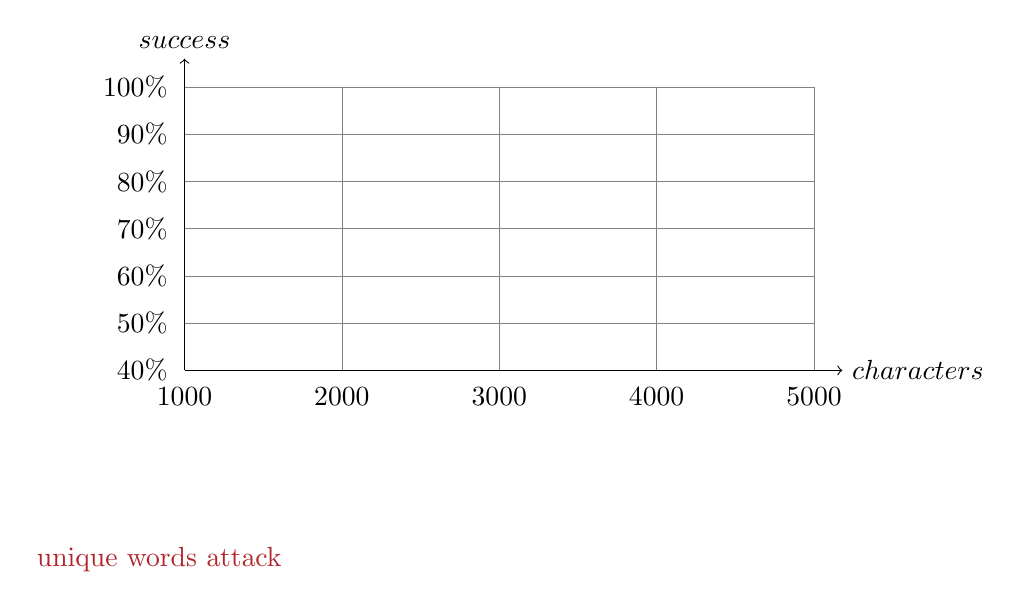
\begin{tikzpicture}[x=0.002cm,y=0.06cm]
  \def\xmin{1000}
  \def\xmax{5000}
  \def\ymin{40}
  \def\ymax{100}
  \draw[style=help lines, ystep=10, xstep=1000] (\xmin,\ymin) grid
  (\xmax,\ymax);
  \draw[->] (\xmin,\ymin) -- (\xmax+180,\ymin) node[right] {$characters$};
  \draw[->] (\xmin,\ymin) -- (\xmin,\ymax+6) node[above] {$success$};
  \foreach \x in {1000,2000,...,5000}
    \node at (\x,\ymin-1.5) [below] {\x};
  \foreach \y in {40,50,...,100}
    \node at (\xmin-45,\y) [left] {\y \%};
  \draw[color={rgb:red,221;green,45;blue,54}] plot[smooth,tension=0.3,mark=*,mark size=1pt] file {data/Monoalphabetic-unique_words.dat}
   node [right] {unique words attack};
\end{tikzpicture}
\caption{Úspěšnost útoku unikátními slovy na monoalfabetickou šifru}
\end{figure}

\subsubsection{Útok pomocí frekvenční analýzy}


\vspace*{\fill}

\noindent
Zdroje ke \ref{monoalphabetic-section}. kapitole: \cite{substitutionwiki}, \cite{monoalphabeticwiki}, \cite{singh2009}

\newpage


%%%% Transposition %%%%
\section{Sloupcová transpozice}
\label{transposition-section}
%

\subsection{Historie}
Záznamy o~použití transpozičních šifer sahají až do 7.~století před naším letopočtem. Tehdy se v~Řecku využíval válec zvaný Skytalé. Na válec se namotal pásek kůže nebo pergamenu, na který se poté napsala zpráva. Po odmotání má výsledný zašifrovaný text přeházené pořadí znaků. Zmínky o~Skyleté sahají sice daleko, ale první dochovalý popis fungování je až z~1.~století našeho letopočtu~\cite{scytalewiki}.

Skytalé je primitivní předchůdce jednoduché sloupcové transpozice. Dá se simulovat jednoduchou sloupcovou transpozicí tak, že použijeme klíč s~abecedně seřazenými písmeny.

\begin{figure}[htbp]
\centering
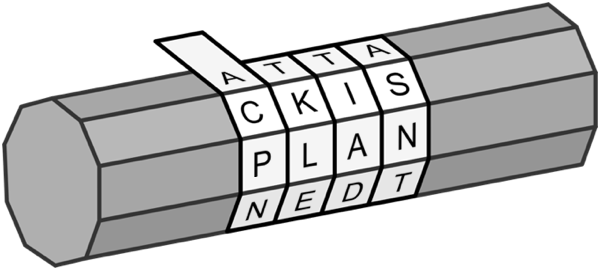
\includegraphics[scale=0.4]{graphics/skytale.png}
\caption{Skytalé}
\end{figure}

\subsection{Popis algoritmu}
První si písmena otevřeného textu poskládáme do obdelníku (tabulky). Pro klíč o~délce $n$~bude mít každý řádek právě $n$~znaků otevřeného textu. První řádek prvních $n$~znaků textu, druhý řádek dalších $n$~znaků atd. Pokud na poslední řádek nevýjde $n$~znaků a~řádek tedy nebude úplně zaplněn, doplní se do něj náhodně vygenerovaná písmena.

Poté seřadíme podle abecedy jednotlivé znaky klíče a~způsob zpřeházení si zapamatujeme. Například klíč \uv{sen} se podle abecedy seřadí na \uv{ens} a~způsob zpřeházení si uložíme jako uspořádanou n-tici $(1, 2, 0)$. Stejným způsobem pak uspořádáme každý řádek. Tabulku přečteme po sloupcích a~to je náš výsledný zašifrovaný text.

Klíče skládající se z~abecedně seřazených písmen nebo klíče o~jednom znaku neposkytují žádné zpřeházení. Pro klíče délky 5 a~víc s~právě jedním přehozením písmen (např \uv{abdce}) je zašifrovaný text také dá bez větší námahy prolomit.

\subsubsection{Příklad}
Chceme zašifrovat zprávu \uv{Smích chytré lidi léčí, blbce uráží} klíčem \uv{werich}. První z~textu odstraníme vše kromě písmen (mezery, tečky, čárky a~diakritiku). Poté text zarovnáme do obdelníku, a~protože do úplného zaplnění chybí na posledním řádku jeden znak, doplní se náhodné písmeno:

\begin{center}
\begin{tabular}{ c c c c c c }
  w & e & r & i & c & h \\ \hline \hline
  s & m & i & c & h & c \\
  h & y & t & r & e & l \\
  i & d & i & l & e & c \\
  i & b & l & b & c & e \\
  u & r & a & z & i & f \\
\end{tabular}
\end{center}

Písmena v~klíči seřadíme podle abecedy, permutace zpřeházení je $(4, 1, 5, 3, 2, 0)$. Stejným způsobem seřadíme sloupce.

\begin{center}
\begin{tabular}{ c c c c c c }
  c & e & h & i & r & w \\ \hline \hline
  h & m & c & c & i & s \\
  e & y & l & r & t & h \\
  e & d & c & l & i & i \\
  c & b & e & b & l & i \\
  i & r & f & z & a & u \\
\end{tabular}
\end{center}

Tabulku přečteme zprava po sloupcích. Výsledný zašifrovaný text je \uv{HEECI MYDBR CLCEF CRLBZ ITILA SHIIU}.

\subsection{Výhody}
Zašifrovaný text má stejnou četnost znaků jako text otevřený. Frekvenční analýza nám proto při luštění nijak nepomůže.

Pokud bychom chtěli použít klíč o~$n$~znacích, existuje $n!$ různých klíčů, které text zašifrují navzájem různým způsobem. Pro klíč o 16 znacích to znamená 20922789888000 možných klíčů, takže útok hrubou silou by i~velmi silnému počítači trval nesmyslně dlouho.

\subsection{Nevýhody}
Proces šifrování ručně je zdlouhavý a nemáme žádnou zrychlovací pomůcku. Pouze pro základní transpozici lze použít Skytalé (popřípadě hranatou tužku nebo jiný válec).

Z délky textu lze jednoduše vypočítat možné délky klíče. Délka klíče musí totiž vždy být dělitel délky textu. Tuto slabost šifry řeší modifikace šifrovacího algoritmu s neúplnou tabulkou (\ref{transpozice-s-neuplnou-tabulkou}).

Mnoho různých klíčů šifruje stejným způsobem. Znaky klíče se totiž můžou abecedně uspořádat stejným způsobem. Například klíče \uv{argo}, \uv{wzxy} a~\uv{adbc} zašifrují text stejně. Při luštění pak stačí vyzkoušet pouze jeden z nich.

Pro krátké klíče je lehce prolomitelná hrubou silou. Pokud bychom předpokládali, že klíč má minimálně 2 a maximálně 5 znaků, znamenalo by to vyzkoušet $2! + 3! + 4! + 5!$, tedy $152$ možných klíčů (včetně slabých), což je prolomitelné i~pro ruční luštění s~tužkou a~papírem.




\subsection{Prolamování}
\subsubsection{Útok nalezením slova v řádku}
Zvolíme si minimální a maximální délku hledaného slova (klíče). Z délky zašifrovaného textu vypočítáme všechny možné dělitele a z výsledné množiny vezmeme pouze ty dělitele, kteří splňují minimální a maximální délku. Tyto čísla uložíme do pole \texttt{keyLengths}. Nyní známe všechny možné délky klíče, protože při procesu šifrování se otevřený text zarovnává do tabulky. 

Pro každé $n$ z \texttt{keyLengths} rozdělíme zašifrovaný text na $n$ částí, kde každá část má počet znaků rovný $(length / n)$, kde $length$ značí délku zašifrovaného textu. Tyto části zarovnáme jako sloupce svisle vedle sebe a budeme je postupně číst po řádcích. Každý řádek má přesně $n$ znaků.

Nyní se snažíme nalézt takový řádek, který se skládá ze stejných písmen jako některé slovo ze seznamu slov zvoleného jazyka, který máme k dispozici. Z takového seznamu získáme pouze ty slova, které mají délku $n$. Program porovná všechny slova tak, že každé slovo rozloží na setřízené pole znaků a až tyty pole porovná. Nalezené dvojice slov skládajících se ze stejných znaků si uložíme do slovníku \texttt{foundPairs} ve tvaru (slovo ze seznamu slov -> řádek šifrovaného textu). To se v cyklu zopakuje pro každé $n$ z \texttt{keyLengths}. Nyní máme v \texttt{foundPairs} všechny nalezené dvojice.

Pro každou dvojici slov z \texttt{foundPairs} zjistíme, jaké přeházení znaků bylo potřeba k transformaci slova ze slovníku na slovo šifrovaného textu. Způsob přeházení (permutaci), např. $[0, 3, 1, 2]$, přidáme do pole \texttt{letterOrders}. Ze všech zjištených permutací v \texttt{letterOrders} vymažeme duplicity, které se mohly objevit. Např. klíče \uv{adbc} a \uv{jzkl} při šifrování přehází pořadí znaků stejným způsobem. Permutace v \texttt{letterOrders} nyní reprezentují možné klíče. Převedeme je na řetězce znaků následovně:

Každé číslo z permutace nahradíme vzorem z množiny znaků písmen tak, že číslo 0 se zobrazí na znak 'a', číslo 1 na znak 'b' atd. Např. pro permutaci $[0, 3, 1, 2]$ vytvoříme klíč \uv{adbc}. Výsledný klíč přidáme do pole \texttt{possibleKeys} a totéž provedeme pro každou permutaci. Nakonec máme v proměnné \texttt{possibleKeys} uloženy všechny pravděpodobné klíče.

Z klíčů v \texttt{possiblePairs} vybereme jako nejpravděpodobnější ten klíč, po jehož rozšifrování textu nalezneme v textu nejvíce reálných slov ze seznamu nejpoužívanějších slov jazyka, který máme k dispozici. Algoritmus vrací právě takový nejpravděpodobnější klíč. Úspěšnost algoritmu ukazuje graf na obrázku \ref{graf-transpozice-hledanislova}.

\begin{figure}[htbp]
\centering
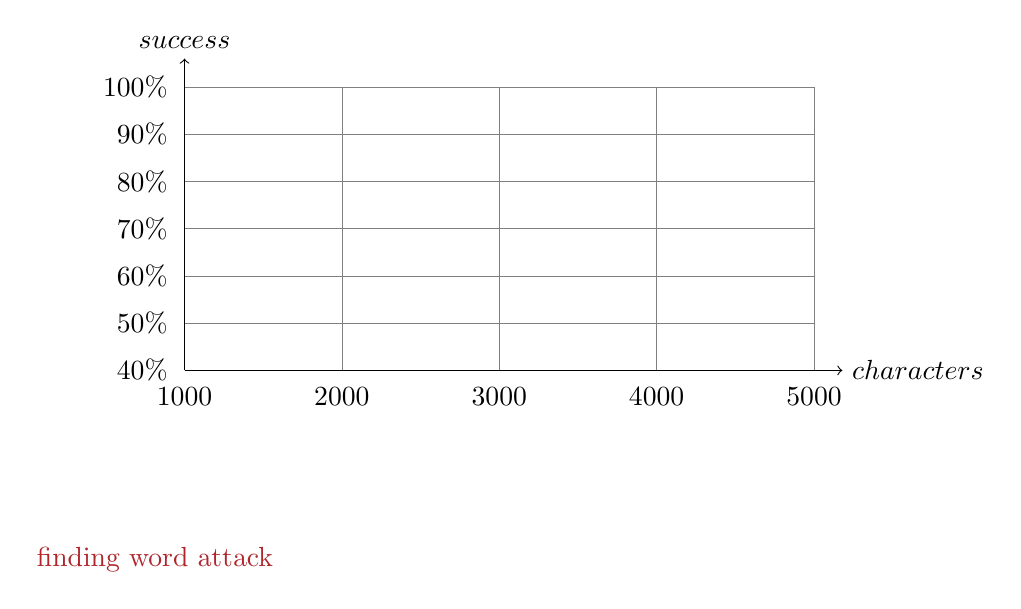
\begin{tikzpicture}[x=0.002cm,y=0.06cm]
  \def\xmin{1000}
  \def\xmax{5000}
  \def\ymin{40}
  \def\ymax{100}
  \draw[style=help lines, ystep=10, xstep=1000] (\xmin,\ymin) grid
  (\xmax,\ymax);
  \draw[->] (\xmin,\ymin) -- (\xmax+180,\ymin) node[right] {$characters$};
  \draw[->] (\xmin,\ymin) -- (\xmin,\ymax+6) node[above] {$success$};
  \foreach \x in {1000,2000,...,5000}
    \node at (\x,\ymin-1.5) [below] {\x};
  \foreach \y in {40,50,...,100}
    \node at (\xmin-45,\y) [left] {\y \%};
  \draw[color={rgb:red,221;green,45;blue,54}] plot[smooth,tension=0.3,mark=*,mark size=1pt] file {data/Transposition-finding_word.dat}
   node [right] {finding word attack};
\end{tikzpicture}
\caption{Úspěšnost útoku nalezením slova v řádku na transpoziční šifru}
\label{graf-transpozice-hledanislova}
\end{figure}

\subsubsection{Útok hrubou silou pomocí reálných slov}
Pokud byl text zašifrován krátkým klíčem, můžeme využít útok hrubou silou a spočítat počet reálných slov. Algoritmus  v prvním kroku zjistí všechny možné délky klíče a uloží je do proměnné \texttt{keyLengths}. Pro každé $n$ z \texttt{keyLengths} vytvoříme množinu čísel $\{0, 1, ..., n-1\}$ a pro každou permutaci takové množiny vytvoříme klíč pomocí známé funkce (0 $\rightarrow$ 'a', 1 $\rightarrow$ 'b', ... , 25 $\rightarrow$ 'z'). Všechny takto vytvořené klíče uložíme do proměnné \texttt{possibleKeys}.

V cyklu projdeme každý klíč z \texttt{possibleKeys} a vyzkusíme jím rozšifrovat zašifrovaný text. Rozšifrovaný text následně projdeme a hledáme výskyt slov ze seznamu nejčastěji používaných slov jazyka, který máme k dispozici. Úspěšnost aktuálně testovaného klíče určíme jako počet takových nalezených slov. Ze všech klíčů vybereme pouze ten nejúspěšnější.

Proces opakujeme pro každou možnou délku klíče $n$ z proměnné \texttt{keyLengths}. Jako odhadnutý použitý klíč vrátíme ten nejúspěšnější z nich. 

Algoritmus testuje všechny permutace, a proto je velmi neefektivní pro dlouhé klíče. Testováním jsem zjistil, že v rozumném čase lze hledat klíče do délky 7 znaků. Úspěšnost algoritmu ukazuje graf na obrázku \ref{graf-transpozice-hrubousilou} na straně \pageref{graf-transpozice-hrubousilou}. Při měření jsem počítal s tím, že náhodně generované klíče mají délku nanejvýš 7 znaků. 

\begin{figure}[htbp]
\centering
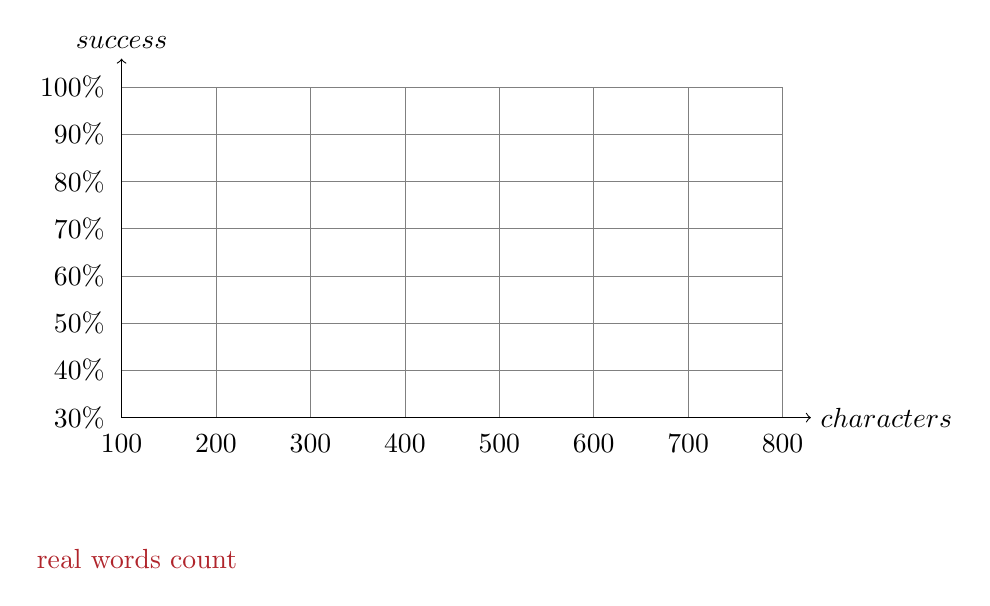
\begin{tikzpicture}[x=0.012cm,y=0.06cm]
  \def\xmin{100}
  \def\xmax{800}
  \def\ymin{30}
  \def\ymax{100}
  \draw[style=help lines, ystep=10, xstep=100] (\xmin,\ymin) grid
  (\xmax,\ymax);
  \draw[->] (\xmin,\ymin) -- (\xmax+30,\ymin) node[right] {$characters$};
  \draw[->] (\xmin,\ymin) -- (\xmin,\ymax+6) node[above] {$success$};
  \foreach \x in {100,200,...,800}
    \node at (\x, \ymin-1.5) [below] {\x};
  \foreach \y in {30,40,...,100}
    \node at (\xmin-7.5,\y) [left] {\y \%};
  \draw[color={rgb:red,221;green,45;blue,54}] plot[smooth,tension=0.3,mark=*,mark size=1pt] file {data/Transposition-real_words.dat}
   node [right] {real words count};
\end{tikzpicture}
\caption{Úspěšnost útoku hledáním reálných slov na transpoziční šifru}
\label{graf-transpozice-hrubousilou}
\end{figure}

\subsection{Variace sloupcové transpozice}
\subsubsection{Jednoduchá sloupcová transpozice s neúplnou tabulkou}
\label{transpozice-s-neuplnou-tabulkou}
Algoritmus šifrování je stejný jako u~klasické jednoduché sloupcové transpozice, až na doplnění náhodných písmen na posledním řádku sestavené tabulky. Ty se nechají prázdné a~tedy ne každý sloupec má stejnou výšku. Šifra se takto stává bezpečnější, protože odstraňuje slabinu jednoduše zjistitelné délky klíče.

\subsubsection{Dvojitá sloupcová transpozice}
Pravidla šifrování se oproti jednoduché sloupcové transpozici nemění. Jediný rozdíl oproti obyčejnému postupu je, že se  text zprávy zašifruje jednoduchou sloupcovou transpozicí dvakrát po sobě. Na druhý krok může být použit stejný nebo rozdílný klíč. Dvojitá transpozice zvyšuje bezpečnost a~množství možných klíčů, obzvlášť při volbě rozdílných klíčů. Rozšifrování se provede obdobně jako u~jednoduché transpozice, ale použité klíče se musí pochopitelně zadat v opačném pořadí. Množství použitých klíčů teoreticky můžeme ještě navýšit.

\subsubsection{Myszkowskiho transpozice}
Tuto modifikaci sloupcové transpozice navrhl francouzský plukovník Émile Victor Théodore Myszkowski v~knize \textit{Cryptographie indéchiffrable} z~roku 1902. Řeší problém opakujících se písmen v klíči. Z~těch sloupců tabulky, které spadají pod stejná písmena klíče, se znaky čtou postupně po sobě. Například pro klíč \uv{lampa} zašifrujeme text \uv{věci na stole} následovně:

\begin{center}
\begin{tabular}{ c c c c c }
  l & a & m & p & a \\ \hline \hline
  v & e & c & i & n \\
  a & s & t & o & l \\
  e & x & g & r & y \\
\end{tabular}
 \qquad \vline \qquad \enspace
\begin{tabular}{ c c c c c }
  a & a & l & m & p \\ \hline \hline
  e & n & v & c & i \\
  s & l & a & t & o \\
  x & y & e & g & r \\
\end{tabular}
\end{center}
	
První dva sloupce uspořádané tabulky (vpravo) pak přečteme jako jeden. Zašifrovaný text bude \uv{EN SL XY VAE CTG IOR}.

\subsubsection{Transpoziční mřížka}
Mřížka je předmět, který má libovolné množství nepravidelně rozmístěných děr. Šifrování probíhá tak, že se znaky otevřeného textu zapisují do otvorů v mřížce a~jakmile jsou všechny vyplněny, mřížka se posune a proces se opakuje. Zbylé prázdné místa (kde mřížka neměla otvor) se poté vyplní náhodně zvolenými znaky. Čím méně děr v~mřížce je, tím je sice šifra bezpečnější, ale výsledná zpráva delší. Další varianta šifry mřížku neposouvá, ale otáčí o~určitý úhel (čtverec o 90\degree , šestiúhelník o 60\degree , atd). Obě strany šifrované komunikace musí sdílet tutéž mřížku. 

\begin{figure}[htbp]
\centering
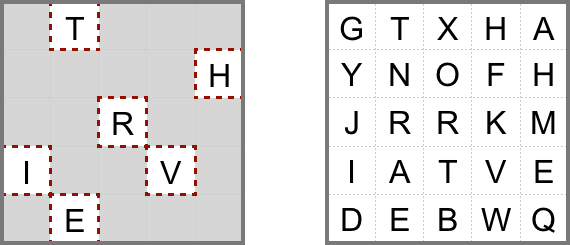
\includegraphics[scale=0.4]{graphics/transposition_table.png}
\caption{Zašifrování slova transpoziční mřížkou}
\label{transposition-table}
\end{figure}

\subsubsection{Primitivní transpozice}
Jeden z~nejjednodušších způsobů transpozice je obyčejné zapsání otevřeného textu do obdelníku a přečtení po sloupcích. Klíč takového šifrovaní je předem dohodnutý způsob zapsání do obdelníku. Kromě klasického po řádcích můžeme použít například spirálu a~další.

\begin{figure}[htbp]
\centering
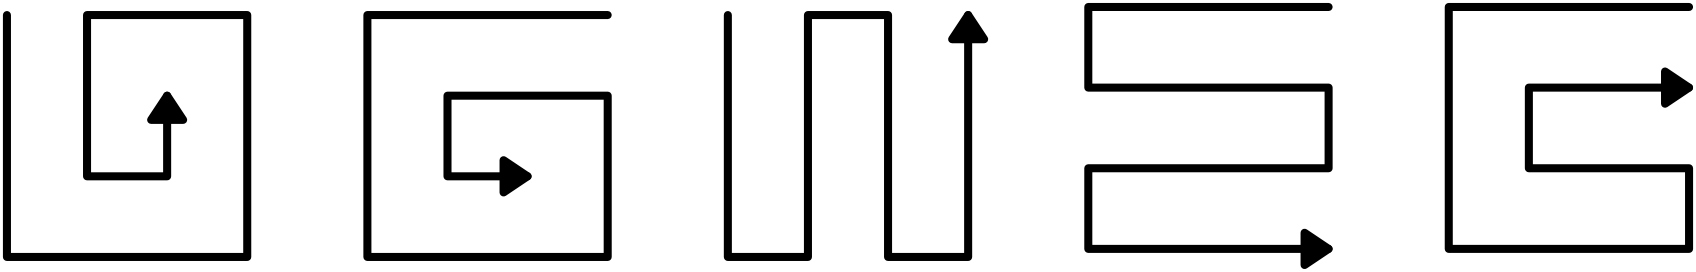
\includegraphics[scale=0.2]{graphics/routes.png}
\caption{Trasy pro zapsání textu}
\label{transposition-routes}
\end{figure}

Opačný způsob využívá trasová transpoziční šifra (route šifra). Text se do obdelníku zapíše vždy stejně a~poté se přečte specifickým způsobem (trasou). Trasy na obrázku \ref{transposition-routes} ukazují jen základní možnosti, jejich kombinacemi se dají vymyslet i~daleko složitější.


\vspace*{\fill}

\noindent
Zdroje k \ref{transposition-section}. kapitole: \cite{transpositionwiki}, \cite{columntranspositionwiki}, \cite{transpositionwiki-en}, \cite{singh2009}

\newpage


%%%% Application %%%%

%%%% User manual %%%%
\section{Uživatelská příručka}
Praktickou část bakalářské práce představuje mobilní aplikace na operační systém iOS od firmy Apple. Aplikace je napsána v~prostředí Xcode 7.2 v~jazycích Objective-C a~Swift 2 a~k~běhu vyžaduje systém iOS ve verzi minimálně 8.1.

Aplikace je rozdělena na čtyři části. První část se zabývá kryptografií, slouží k~šifrování a~dešifrování vloženého textu. V druhé části lze vyzkoušet kryptoanalytické útoky na vložený zašifrovaný text. Třetí část je výuková a snaží se popsat historii a~chování šifry, ukázat šifrování na příkladech a~vysvětlit možnou kryptoanalýzu. Poslední čtvrtá část je nastavení aplikace, slouží k~výběru šifry, kryptoanalytického útoku na ní a~výběru jazyka, s~kterým algoritmy budou pracovat.

\subsection{Kryptografická část}
\label{app-encryption-section}
Záložka \uv{Encryption} slouží k~provádění šifrování a~dešifrování textu. 

\begin{figure}[htbp]
\centering
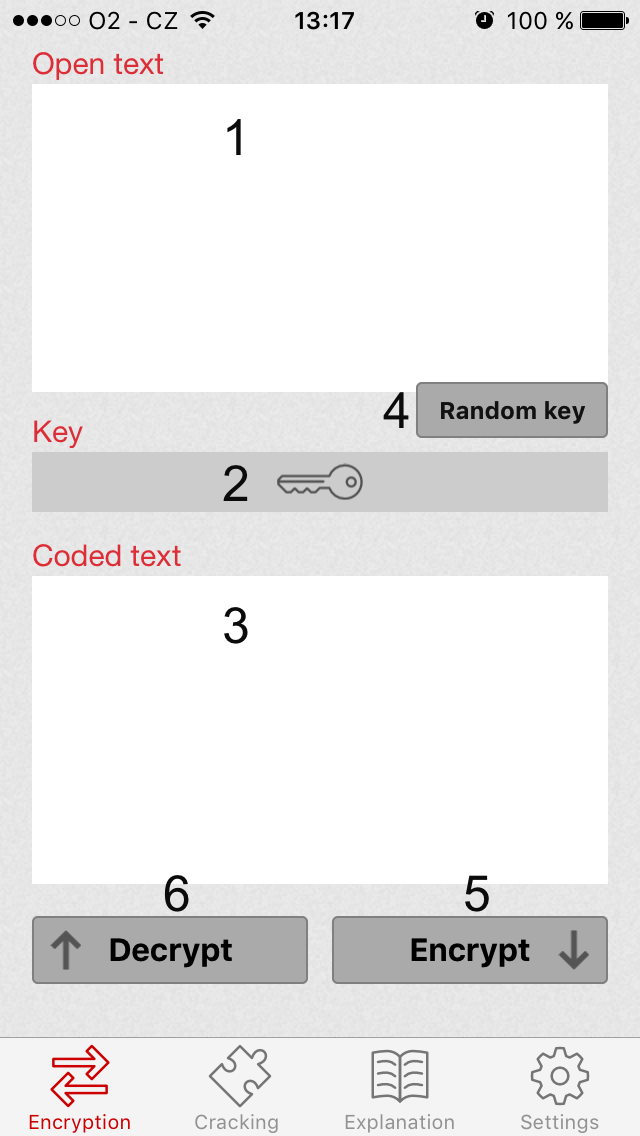
\includegraphics[scale=0.32]{graphics/app/encryption.png}
\caption{Aplikace - kryptografická část}
\label{app-encryption}
\end{figure}

\newpage

Jednotlivé ovládací prvky jsou:
\begin{enumerate}
  \item Textové pole pro otevřený text. Uživatel zde může vkládat text určený k~zašifrování.
  \item Textové pole pro klíč. Uživatel do něj může klíč napsat nebo vygenerovat tlačítkem \texttt{Random key} (4). Pokud je pole prázdné nebo klíč není validní k~momentálně zvolené šifře a~uživatel se snaží šifrovat, vyskočí dialogové okno s~chybovou hláškou.
  \item Textové pole pro zašifrovaný text. Uživatel zde může vkládat text určený k~rozšifrování.
  \item Tlačítko pro vložení náhodného klíče. Po stisknutí se podle momentálně zvolené šifry vygeneruje náhodný klíč a vloží se do textového pole \texttt{Key} (2).
  \item Tlačítko pro zašifrování zprávy. Vezme se otevřený text z~textového pole \texttt{Open text}~(1), zašifruje se momentálně zvolenou šifrou a~klíčem z~pole \texttt{Key} (2) a výsledek se vloží do textového pole \texttt{Coded text} (3).
  \item Tlačítko pro rozšifrování zprávy. Vezme se zašifrovaný text z~textového pole \texttt{Coded text}~(3), rozšifruje se momentálně zvolenou šifrou a~klíčem z~pole \texttt{Key} (2) a výsledek se vloží do textového pole \texttt{Open text} (1).
\end{enumerate}

\subsubsection{Příklad použití}
V~této záložce může uživatel šifrovat nebo dešifrovat text zvoleným klíčem. Pro šifrování vloží otevřený text do pole \texttt{Open text}, napíše klíč do pole \texttt{Key} nebo si ho nechá náhodně vygenerovat tlačítkem \texttt{Random key}. Tlačítko \texttt{Random key} je neviditelné, viditelným se stává až po zaměření textového pole \texttt{Key} a~do neviditelného stavu se vrací se zaměřením na jiný ovládací prvek. Poté uživatel stiskne tlačítko \texttt{Encrypt} a~výsledný zašifrovaný text se zobrazí v~textovém poli \texttt{Coded text}.

Opačný proces pro dešifrování je podobný. Uživatel první vloží zašifrovaný text do pole \texttt{Coded text}, zvolí klíč již popsaným způsobem a~stiskne tlačítko \texttt{Decrypt}, které zašifrovaný text z pole \texttt{Coded text} rozšifruje inverzním šifrovacím algoritmem momentálně zvolené šifry a~vloží jej do pole \texttt{Coded text}.


\subsection{Kryptoanalytická část}
\label{app-cracking-section}
Záložka \uv{Cracking} slouží ke kryptoanalýze. Ovládací prvky jsou stejného typu a~jejich rozložení velmi podobné jako u~předchozí části \ref{app-encryption-section}. 

Textové pole \uv{Coded text} slouží pro vložení zašifrované zprávy, pod ním pole \uv{Guessed key} zobrazuje uhodnutý klíč a~pole \uv{Guessed decryption} zobrazuje text dešifrovaný takovým klíčem. Celý proces kryptoanalýzy spustí tlačítko \uv{Crack} (český překlad: prasknout, rozluštit, rozbít, vyřešit).

Textová pole \uv{Guessed key} a \uv{Guessed decryption} zůstávají nepřístupná (disabled) dokud neskončí kryptoanalýza. Po dokončení útoku se odemknou, aby si uživatel mohl popřípadě zkopírovat výsledek.

\begin{figure}[htbp]
\centering
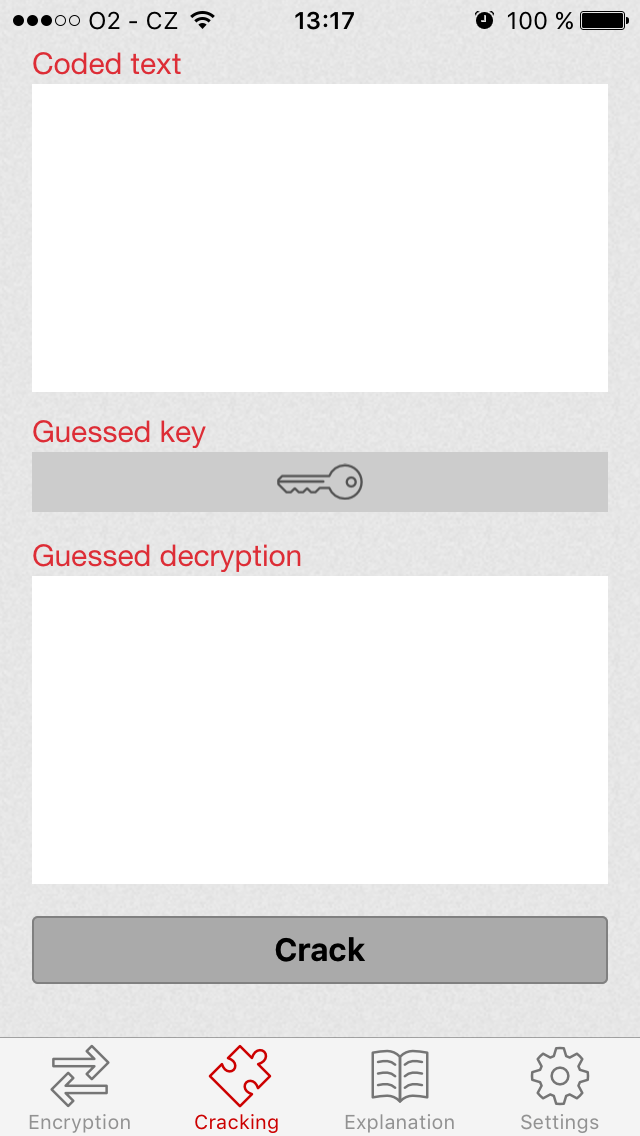
\includegraphics[scale=0.32]{graphics/app/cracking.png}
\caption{Aplikace - kryptoanalytická část}
\label{app-cracking}
\end{figure}

\subsubsection{Příklad použití}
Uživatel chce rozšifrovat zašifrovanou zprávu a~nezná klíč. Zprávu vloží do textového pole \texttt{Coded text} a~stiskne tlačítko \texttt{Crack}. Spustí se zvolený prolamovací algoritmus nad vloženým textem. Podle typu šifry a útoku může výpočet trvat různou dobu. Po dokončení se do textového pole \texttt{Guessed key} vloží uhodnutý klíč a~do pole \texttt{Guessed decryption} zpráva rozšifrovaná tímto klíčem.


\subsection{Učební část}
\label{app-explanation-section}
Tato část slouží k~vysvětlení zvolené šifry. Jedná se o~stručný popis historie a~fungování šifry, včetně pomocných obrázků, příkladů a~popisu kryptoanalýzy.

Informací je většinou tolik, že se na jednu obrazovku zařízení nevejdou. Standartním posunem dolů (drag and drop) se uživatel dostane ke všem sekcím.

\begin{figure}[htbp]
\centering
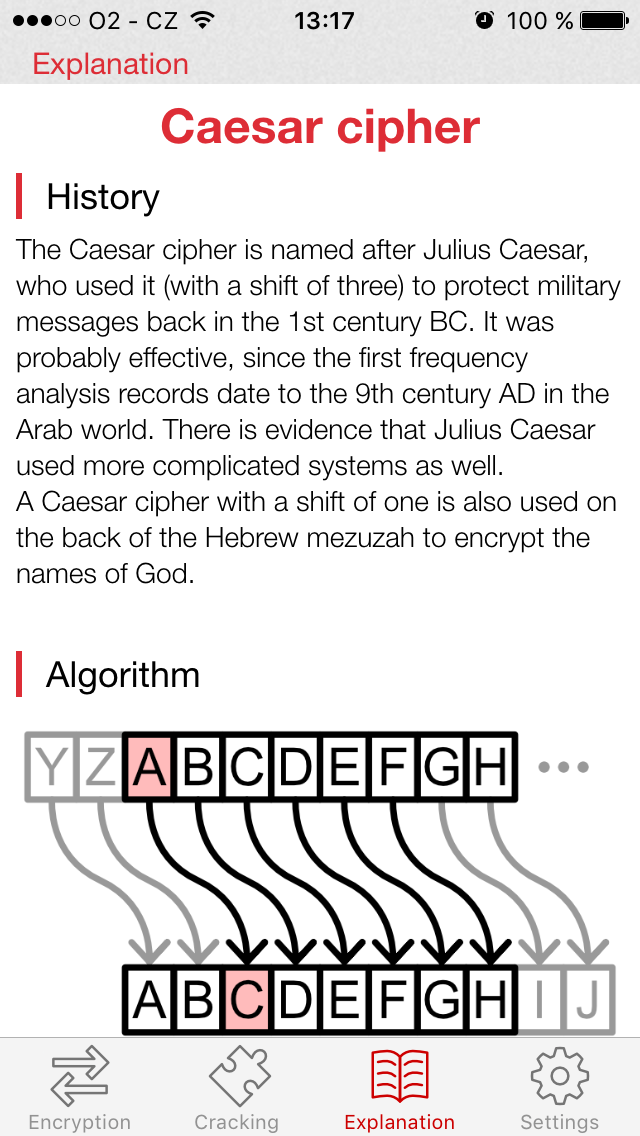
\includegraphics[scale=0.32]{graphics/app/explanation.png}
\caption{Aplikace - učební část}
\label{app-explanation}
\end{figure}

\subsection{Nastavení}
\label{app-settings-section}
V žáložce nastavení si uživatel volí šifru, útok na ni a dodatečné informace o jazyku. Šifru, s~kterou chce pracovat, zvolí ze seznamu v~ovládacím prvku s~nadpisem \texttt{Choose cipher}. 

Po zvolení šifry se v~seznamu ovládacího prvku s~nadpisem \texttt{Type of attack} vypíšou možné útoky na zvolenou šifru s~defaultně zvolenou první z~nich.

Po kliknutí na tlačítko \texttt{Language statistics} vyjede seznam přístupných jazyků, z~kterých si uživatel jeden zvolí. Zvolená statistika jazyka slouží k~prolamování, využije se tedy jen na záložce \ref{app-cracking-section}.

Obrázky \ref{app-settings} ukazují prostředí záložky nastavení a teké~seznam zvolitelných statistik jazyka.

Na spodu záložky je malé tlačítko \texttt{About this app}, po jejímž stisknutí vyjede lišta se stručnými informacemi o~aplikaci a~jejím účelu.
\\

\begin{figure}[htbp]
\centering
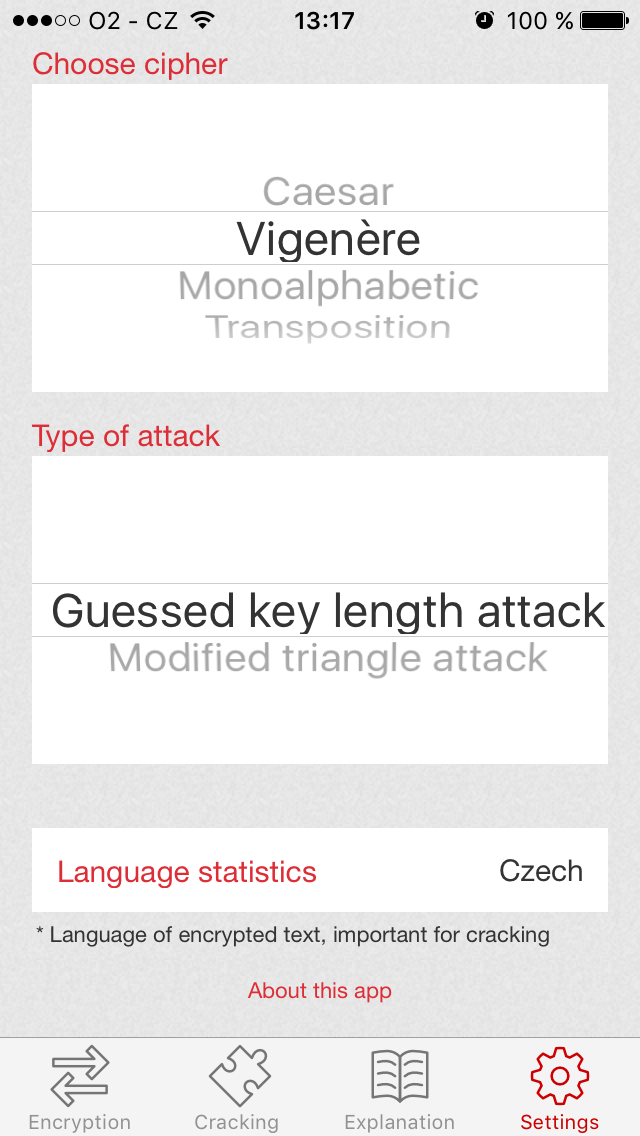
\includegraphics[scale=0.3]{graphics/app/settings.png}\qquad 
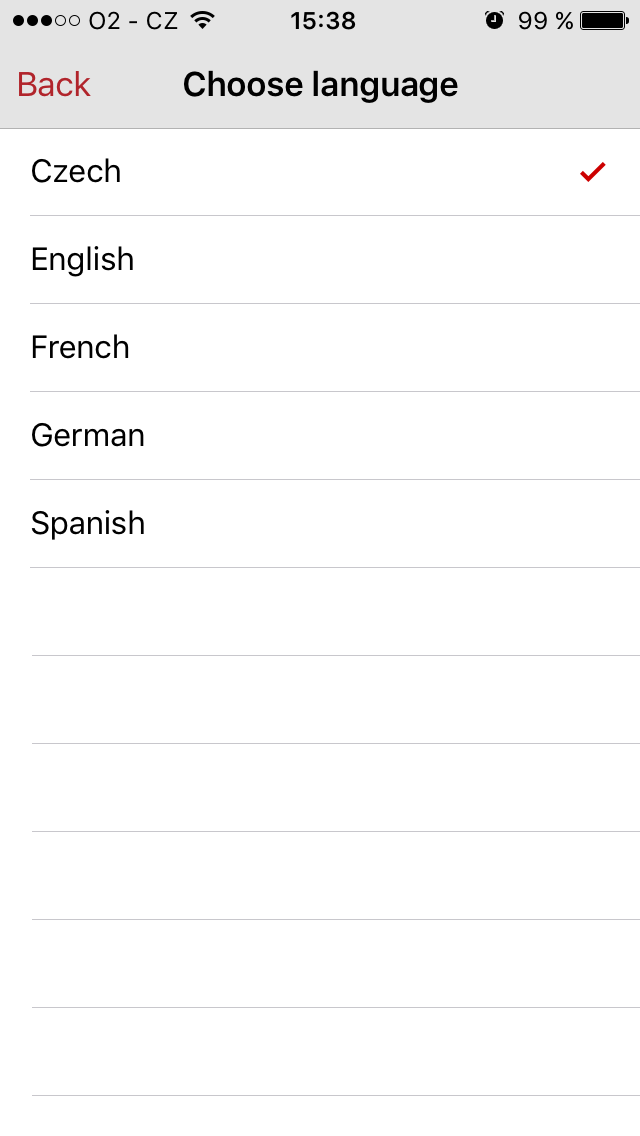
\includegraphics[scale=0.3]{graphics/app/languages.png}
\caption{Aplikace - nastavení (vlevo), volba statistiky jazyka (vpravo)}
\label{app-settings}
\end{figure}





\newpage

%%%% Code documentation %%%%
\section{Dokumentace zdrojového kódu}
Aplikace je napsána ve dvou programovacích jazycích a ukazuje jejich jednoduchou integraci. Ve starším z~jazyků, Objective-C, jsou napsány všechny kryptografické a kryptoanalytické algoritmy pracující pouze s~textem. Ve druhém jazyku, Swift 2, je napsáno grafické uživatelské rozhraní (GUI).

\subsection{Ciphers}
Obsahuje všechny algoritmy pro šifrování a dešifrování jednotlivých šifer. Každá šifra je samostatná třída implementující protokol \texttt{Cipher}, který udává povinné metody. Mezi ně patří šifrování, rozpoznání validního klíče a~generování náhodného klíče.

Jednotlivé třídy šifer se jmenují \texttt{Caesar}, \texttt{Vigenere}, \texttt{Monoalphabetic} a~\texttt{Transposition}. Každá z~nich obsahuje vlastní pomocné algoritmy potřebné k~šifrování a~dešifrování.


\subsection{Cracking}
Obsahuje algoritmy kryptoanalytických útoků a~k~nim pomocné algoritmy analyzující zašifrovaný text. Podobně jako u~\texttt{Ciphers} se tu využívá protokol \texttt{Crack} a~všechny třídy jej implementují.

Jednotlivé třídy na prolamování jsou \texttt{CaesarCrack}, \thinspace \texttt{VigenereCrack}, \thinspace\texttt{MonoalphabeticCrack} a~\texttt{TranspositionCrack}. 


\subsection{Utilities}
Obsahuje všechny dodatečné třídy a~metody, které pomáhají zpracovat text, analyzovat text a~provádět složitější matematické operace.

Třída \texttt{Combinatorics} implementuje kombinatorické algoritmy pro permutace a~variace nad textovými řetězci a~znaky v~nich.

Třída \texttt{FileReader} implementuje pomocnou strukturu pro lepší práci s~textovými soubory jako například jednoduché čtení po řádcích. Stejně tak třída \texttt{LanguageParser} implementuje parser pro XML soubory z \texttt{Languages}, které obsahují statistické informace o~jazycích.

Poslední je třída \texttt{Utils}, ve které se nachází metody pro prácí s textem (normalizace textu, smazání bílých mezer na konci řetězců atp.), metody pro spočítání četnosti znaků a~četnosti reálných slov. Dále metody pro hledání dělitelů a~pro inicializaci často používaných strukutur.


\subsection{Storage}
Obsahuje třídy, díky nímž se aplikace dostává k~datům potřebným při prolamování nebo při výpisu dostupných šifer. Dále obsahuje textové soubory slovníků všech slov a~slovníků unikátních slov. Ve složce \texttt{Languages} jsou navíc XML soubory se statistikami jazyka.

Třida \texttt{Storage} implementuje metody například pro získání všech dostupných šifer, pro získání filereaderů jednotlivých slovníků všech slov nebo filereaderů souborů se seznamem unikátních slov.

Třída \texttt{Language} obsahuje metody pro získání předpokládané frekvence písmen jazyka, nejčastějších bigramů, trigramů a~celých slov. Dále umožňuje nastavit zvolený jazyk a~načíst potřebné struktury.


\subsection{Explanations}
Tato složka obsahuje HTML soubory s~informacemi o~jednotlivých šifrách. Ke každé šifře je jeden takový soubor, který dodržuje jednoduchou strukturu nadpisů a~odstavců. Přiložen je také CSS soubor \texttt{styles.css} pro nastylování vzhledu elementů a~použité obrázky ve složce \texttt{img/}.

\subsection{ViewControllers}
Obsahuje všechny ViewControllery pro GUI aplikace. Každé okno má svůj ViewController obsluhující události, které mohou nastat. 

Třída \texttt{EncryptionViewController} obsluhuje kryptografickou část (první zleva ze spodních záložek, viz. \ref{app-encryption-section}), \texttt{CryptanalysisViewController} kryptoanalytickou část (druhá záložka, \ref{app-cracking-section}), \texttt{ExplanationViewController} učební část (třetí záložka, \ref{app-explanation-section}) a~poslední \texttt{SettingsViewController} nastavení (\ref{app-settings-section}).

\texttt{LanguagesTableViewController} a~\texttt{AboutAppViewController} jsou třídy obsluhující vyjížděcí okno na zvolení jazyka a~okno s~informacemi o~aplikaci.


\subsection{Supporting Files}
Zde se nachází soubor \texttt{Bridging-Header.h}, který je nezbytný pro souběh jazyku Objective-C v~aplikaci postavené na jazyku Swift. Jsou v něm sepsané importy všech tříd, které aplikace může použít.

Soubory \texttt{dictionary\_filter.awk} a~\texttt{unique\_filter.awk} jsou krátké AWK programy, které slouží k~filtrování textových souborů se slovníky.




\section{Dodatky}



%% v případě tvorby rejstříku přeložit vygenerovaný soubor .idx
%% programem Makeindex a v případě tvorby seznamu zkratek spustit
%% program Makeglossaries s parametrem jméno souboru zdrojového textu
%% bez přípony a následně opět (dvakrát) přeložit zdrojový text
%% programem pdfLaTeX.


%% Závěry práce. V jazyce práce a anglicky. Text pro jiný než
%% nastavený jazyk práce (nepovinným parametrem language makra
%% \documentclass, výchozí český) se zadává použitím makra s uvedením
%% jazyka jako nepovinného parametru.
\begin{kiconclusions}
-- závěr práce --
\end{kiconclusions}

\begin{kiconclusions}[english]
-- thesis conclusions --
\end{kiconclusions}

%% Přílohy obsahu textu práce, za makrem \appendix.
\appendix

%% \section{První příloha}
%% Text první přílohy


\section{Obsah přiloženého CD} \label{sec:ObsahCD}

\begin{description}

\item[\texttt{Application/}] \hfill \\
  Aplikace \dots
  
\item[\texttt{Images/}] \hfill \\
  Veškerá grafika vytvořená pro použití jak v~aplikaci, tak v~této textové práci. Obsahuje vektorové obrázky včetně rastrových exportů.
  
\item[\texttt{Text/}] \hfill \\
  Tento text bakalářské práce vypracovaný v~sázecím systému \LaTeX
  
\end{description}



\newpage


%% \nocite{*}
\bibliographystyle{plain}
\bibliography{citace}


\end{document}
